\chapter{Experiments}
    The results of the first experiments performed on the LSP facility are presented here. These include an exploration of ignition methods and their reliability, the attempted replication of power-threshold experiments seen in LSP literature, and the analysis of LSP's absorption, heat deposition, and spectral characteristics. Preliminary flowing data is also presented and contrasted with the static case.

    \autoref{fig:finalsetup_static} provides an overview of the instrumentation used in static experiments and their relative positions. \added{All experiments were performed with a 200-mm-focal length lens, focusing the 1-in-wide laser beam to a focus approximately \qty{0.5}{mm} in diameter. These parameters result in an effective f-number of 7.9 for the laser beam. The working fluid is argon, chosen for its safer handling characteristics over hydrogen or nitrogen, as discussed in \autoref{chp:background}.}

    \begin{figure}[h]
        \centering
        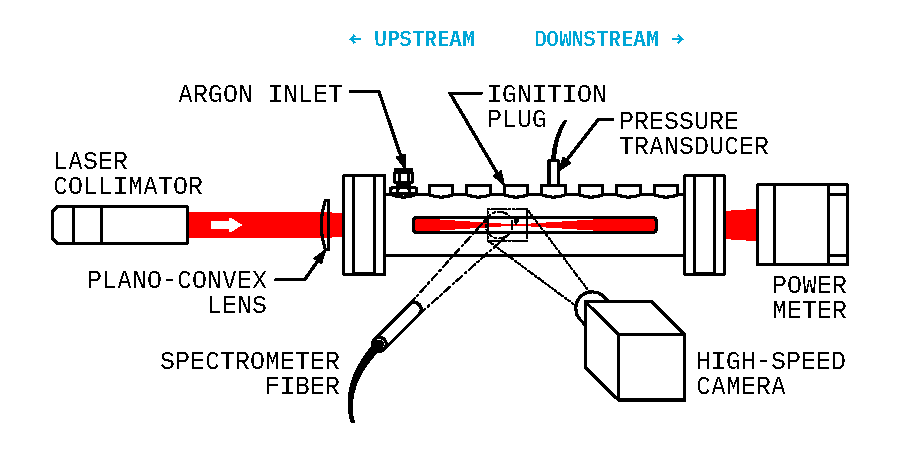
\includegraphics[width=0.85\textwidth]{assets/5 results/finalsetup_static}
        \caption{Static configuration of the test section}
        \label{fig:finalsetup_static}
    \end{figure}

    A summary of the experiments/tests performed, along with their goal and success criteria, is presented in \autoref{tab:experiments}. The experiments performed in this chapter involve one subsystem test (ignition), and the collection of data relevant in studying the laser absorption and heat deposition effectiveness of LSP.

    \begin{table}[h]
        \centering
        \caption{Overview of experiments/tests, goals, and success criteria}
        \label{tab:experiments}
        \newcolumntype{Y}{>{\hsize=.6\hsize\linewidth=\hsize}X}
        \newcolumntype{Z}{>{\hsize=1.2\hsize\linewidth=\hsize\raggedright\arraybackslash}X}
        \renewcommand{\arraystretch}{1.3}
        \begin{tabularx}{\textwidth}{@{}YZY@{}}
            \toprule
            Experiment/Test & Goals & Success criteria \\
            \midrule
            Ignition test & Test and fine-tune ignition methods & 90\% reliability \\
            Power threshold & Identify minimum power needed to sustain plasma for 3--20~bar  & - \\
            Laser absorption & Determine absorption coefficient in agreement with literature/models & - \\
            Heat deposition & Estimate heat deposition using static pressure measurements & - \\
            Spectroscopy & Estimate peak plasma temperature using emission spectrum & - \\
            Flowing experiment & Compare measured data to static case & - \\
            \bottomrule
        \end{tabularx}
    \end{table}

    \section{Preliminary ignition tests} \label{sec:ignitiontest}
        Once the necessary components of the experiment were integrated, a preliminary testing campaign began to attempt to ignite LSP.\added{ Two ignition methods were tested---both are designed to generate a seed cloud of free electrons able to initiate the IB absorption process, which can only sustain itself in ionized argon ($T >$~\qty{1000}{K}).} The hope was to resolve any unforeseen practical issues, then quickly move on to replicating the power threshold experiments of past LSP literature~\cite{zimakovInteractionNearIRLaser2016,matsuiGeneratingConditionsArgon2019,luCharacteristicDiagnosticsLaserStabilized2022}. The test campaign aimed to answer two questions:
        \begin{itemize}
            \item Can LSP be achieved with this experimental setup?
            \item How reliable is LSP ignition with this system?
        \end{itemize}
        To answer these questions, experimental trials would be run in conditions most favorable to steady LSP formation, i.e. at maximum laser power and maximum test section pressure: \qty{3}{kW} and \qty{20}{bar}. Successful ignition would be determined based on two independent measures:
        \begin{enumerate}
            \item The high-speed camera should be able to image the LSP growing and propagating towards the laser source over the course of the laser pulse, as consistently documented in LSP literature.
            \item A measurable drop in laser energy reaching the Gentec power meter should be observed.
        \end{enumerate}
        LSP would only be deemed to have successfully ignited if the expected behavior was observed with both instruments.

        \subsection{Spark ignition} \label{subsec:results_sparkignition}
            Laser alignment was immediately found to be a non-trivial problem. In order to successfully ignite the LSP, the laser must be focused onto the arc generated by the spark igniter. To maximize the chance of ignition, the laser flux at the arc must be as great as possible, so the focused laser dot must be as small as possible. This makes alignment tolerances much stricter, as the laser is less likely to be incident on the thin arc at all.

            Compounding this issue was the fact that the path taken by the arc between both electrode tips was not consistent. As seen in \autoref{fig:sparkAlignment}, the location of the arc was highly variable: although an average arc path could be determined, the arc could form up to \qty{1}{mm} away. This made it impossible to ensure consistent alignment between the arc and the laser focus. This issue could be alleviated by repeatedly triggering the spark, but the smart coil had a nominal delay of \qty{3}{ms} between sparks, only allowing up to three ignition attempts within a single laser pulse, making this approach of little viability for high-power pulse laser tests. Repeated sparks could be used with CW laser operation at \qty{300}{W}, but the lower laser power also reduces the likelihood of successful LSP ignition.

            \begin{figure}[h]
                \centering
                \begin{subfigure}[t]{0.47\textwidth}
                    \centering
                    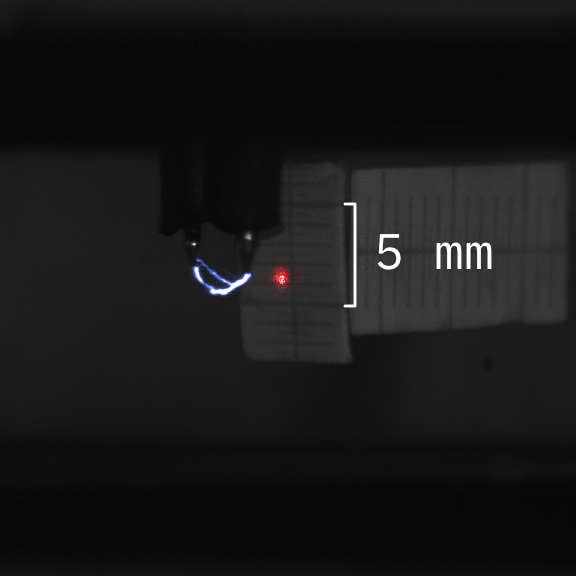
\includegraphics[]{assets/3 design/sparkAlignment_one.jpg}
                    \caption{Single arc generated by the spark igniter}
                    \label{fig:sparkAlignment_one}
                \end{subfigure}
                \hfill
                \begin{subfigure}[t]{0.47\textwidth}
                    \centering
                    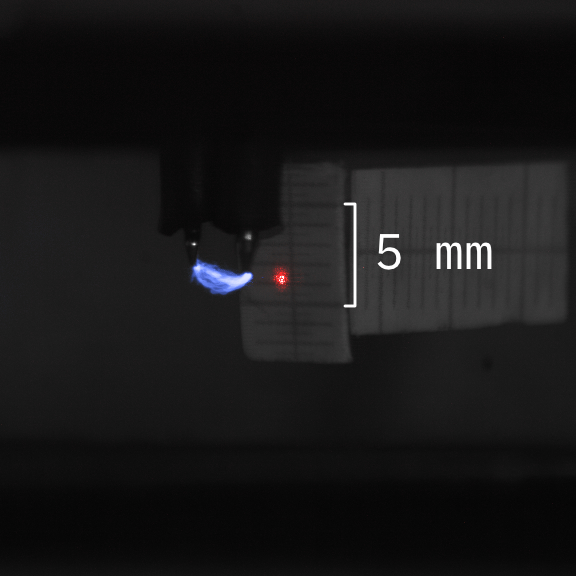
\includegraphics[]{assets/3 design/sparkAlignment.jpg}
                    \caption{Several arcs stacked together to create a ``heatmap'' of arc formation. Note the large variance in the path taken by the arc.}
                    \label{fig:sparkAlignment_heatmap}
                \end{subfigure}
                \caption[Composite photos made during a typical spark--laser alignment procedure]{Composite photos made during a typical spark--laser alignment procedure. The gray-scale background, blue arcs, and red guide laser photos were taken separately then stacked together to be able to compare the relative position of the arcs and laser.}
                \label{fig:sparkAlignment}
            \end{figure}

            In addition, the laser could not be aligned without placing reflecting or scattering material in the beam path. As seen in \autoref{fig:sparkAlignment}, a target must be placed near the ignition point to perform the alignment (and also serves as a scale indicator). However, this alignment target had to be removed to pressurize the test section, which was required both to determine the spark location, and to perform the LSP ignition test. Pressurization cycles and the placing/removal of this target made the alignment process slow and cumbersome. Alignment with the arcs could not be confirmed visually since the target could not be present when pressurizing the test section.

            Despite these difficulties, several attempts were made to ignite LSP with this method, and a few were successful. The first successful test was performed at \qty{10.0}{bar} with a full power pulse (\qty{30.8}{J}). A paper target had been placed next to the electrodes to facilitate alignment, so no measurements were made of the pulse energy transmitted through the plasma for the first few successful tests. However, high-speed footage showed strong evidence of plasma formation: a bright flash saturating the camera sensor, igniting at the time of spark formation, as seen in \autoref{fig:lsp1}. Such a flash had never been observed in past (failed) ignition tests. Although this suggested that some plasma had been formed, there was a possibility that the alignment target\comment[id=AH]{either: alignment of the target or: target alignment}\comment[id=ED]{this is a target (subject) \emph{for} alignment (adj?)} was affecting the experiment and may even have contributed to the ignition. The footage showed evidence of particles being ejected from the area around the ignition point, possibly due to the interaction between the laser, plasma, and the paper target.

            \begin{figure}[h]
                \centering
                \begin{subfigure}[t]{0.32\textwidth}
                    \centering
                    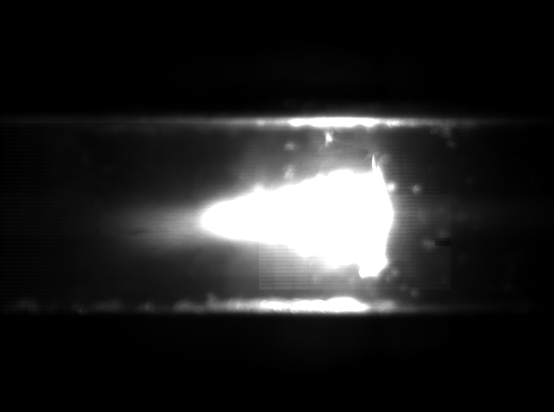
\includegraphics[width=\textwidth]{assets/3 design/LSP1_frames/20.jpg}
                    \caption{2.0~ms}
                    \label{fig:lsp1_20}
                \end{subfigure}
                \hfill
                \begin{subfigure}[t]{0.32\textwidth}
                    \centering
                    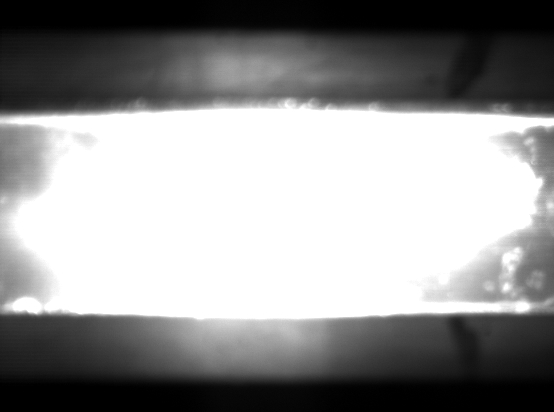
\includegraphics[width=\textwidth]{assets/3 design/LSP1_frames/30.jpg}
                    \caption{3.0~ms}
                    \label{fig:lsp1_30}
                \end{subfigure}
                \hfill
                \begin{subfigure}[t]{0.32\textwidth}
                    \centering
                    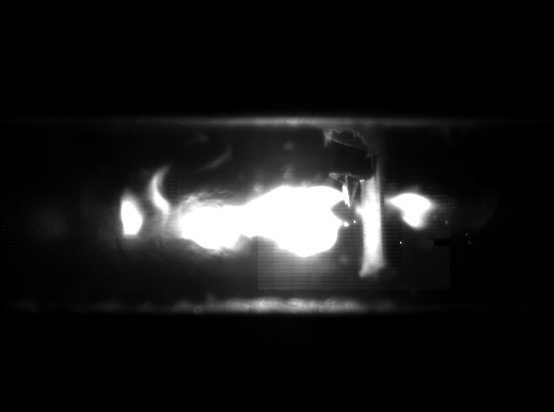
\includegraphics[width=\textwidth]{assets/3 design/LSP1_frames/75.jpg}
                    \caption{7.5~ms}
                    \label{fig:lsp1_75}
                \end{subfigure}
                \caption[High-speed footage frames of first successful LSP ignition]{High-speed footage frames of first successful LSP ignition. The horizontal reflections above and below the event are the edges of the observation window.}
                \label{fig:lsp1}
            \end{figure}

            The experiment was repeated with the target several times, ensuring that the flash was not the result of merely burning a hole through the paper target. In addition, the exposure settings were adjusted (increasing the ND filter to ND2048 and setting the aperture to \textit{f}/22) to provide a clearer view of the brightest part of the frame, the LSP core. A snapshot of the resulting footage is shown in \autoref{fig:lsp3}, revealing a slender plasma core, approximately contained within the focused laser beam (note the thinner right tip of the LSP compared to the left tip). The plasma was observed to grow towards the source of the laser, as reported in the experimental LSP literature. This appearance and growth behavior provided additional evidence that these tests were truly achieving laser-sustained plasma, as opposed to some other phenomenon.

            \begin{figure}[h]
                \centering
                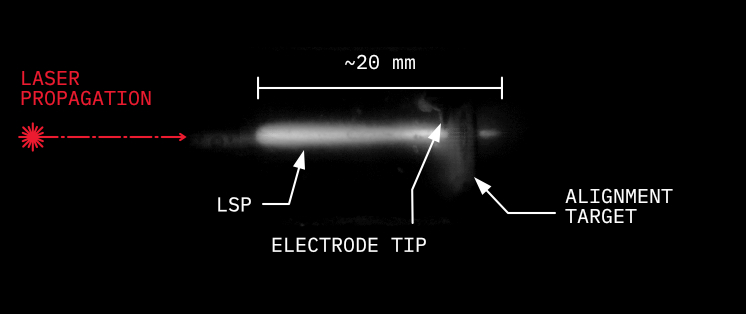
\includegraphics[]{assets/3 design/LSP3_annotated.jpg}
                \caption[Third successful LSP test ignited by arc discharge]{Third successful LSP test ignited by arc discharge. Snapshot from just before the end of the laser pulse. Dimension is approximate.}
                \label{fig:lsp3}
            \end{figure}

            To provide complete confidence that this indeed was LSP, more experiments were performed without the paper target. This allowed the measurement of the laser energy that was not absorbed by the plasma and would confirm that the LSP is ignited purely by the spark, as opposed to ablated material from the paper target. With a fully uninterrupted beam path, the power meter reported a 70 to 80\% drop in laser pulse energy during a test, suggesting that significant laser absorption was occurring in the plasma. This thus satisfied the second criterion for determining successful LSP ignition.

        \subsection{Wire ignition} \label{subsec:results_wireignition}
            As power-threshold experiments were underway, as discussed in \autoref{sec:results_powerthreshold}, it became apparent that the reliability of spark ignition was unsatisfactory. The inability to consistently arc through the laser beam meant that most ignition attempts would fail, especially below full laser power. Reliability of the spark-ignition system was estimated between 10\% and 50\% depending on conditions.

            Private communications with Todd and Nassar (involved in \cite{akarapuNumericalModelLasersustained2009,nassarInvestigationLasersustainedPlasma2012}) highlighted the difficulty of spark ignition, and motivated the change to a solid-target system, with the use of thin metallic wire as an ignition target. \added{As briefly mentioned in \autoref{sec:sparkignition}, this ignition mechanism creates the necessary electron cloud by thermionic emission from the metal target. Metal is heated to a point where thermal energy in the surface overcomes the surface's work function, releasing electrons.} Tungsten had been used successfully in past LSP experiments, such as those of \textcite{toyodaThrustPerformanceCW2002}, so 0.01-in-diameter tungsten wire was acquired and placed in the beam path as a target. \added{Approximately 1~in of wire was protruding from the ignition plug, of which only a $\sim$0.5-mm section was exposed to the laser based on the apparent focal point diameter. Estimates suggested that the local wire temperature would increase to 1500--3000~K within \qty{0.1}{ms}, assuming all laser energy is absorbed ($\approx $\qty{0.3}{J}) in the region exposed to the laser . This estimate suggests a full-power laser pulse is sufficient to trigger thermionic emission, which occurs at temperatures beyond \qty{2000}{K} in tungsten, according to \textcite{awanChapterElectronsNanostructures2020}.}

            Wire ignition proved to be easier to work with, as laser alignment was simpler. However, it did not guarantee ignition either---wire ignition's greater reliability revealed other important factors in consistently achieving LSP:
            \begin{itemize}
                \item Axial positioning of the laser focus such that it coincides with the target is crucial to generate the ``seed'' cloud of electrons necessary for LSP ignition.
                \item Ensuring high argon purity in the chamber was also found to be important. Venting of residual air in the system done by performing several pressurization-vent cycles with argon---at least 3 cycles up to \qty{5}{bar}---before final pressurization to the test pressure. While this was sufficient for tests at \qty{10}{bar} and above, additional cycles were found to improve ignition reliability at low pressures (\qtyrange{3}{10}{bar}).
            \end{itemize}
            Factors that were hypothesized to impact reliability but ultimately were found to have little to no impact include:
            \begin{itemize}
                \item Focusing the laser on the same spot on a wire across several tests
                \item Touching/dirtying the wire before installing it in the test section
                \item Sanding/cleaning the wire before installing it in the test section
            \end{itemize}
            Once these reliability factors were identified and controlled, wire ignition proved to be highly reliable, attaining practically 100\% reliability. \added{At the time of writing, 124 LSPs were successfully ignited, 80\% by wire ignition.}

        \subsection{Early LSP observations}
            These early ignition tests already allowed the observation of LSP. \autoref{fig:ignition_frames} depicts the initial growth of LSP ignited off a tungsten wire, showing rapid growth over a fraction of a millisecond. Under the right ignition conditions, plasma would form practically as soon as the laser was turned on, before the tungsten wire had time to heat up and melt off. This quick ignition would prove to be a useful property when combined with stepped-pulse profiles in later power threshold experiments. \added{In some cases, the wire exhibited signs of localized melting. This observation suggests parts of the wire experienced temperatures beyond tungsten's \num{3700}-\unit{K} melting point~\cite{royalsocietyofchemistryTungstenElementInformation2023}, greater than the temperature estimates of 1500--3000~K. This discrepancy is likely due to the laser beam's non-uniform irradiance profile, exposing small portions of wire to greater laser fluxes than the average flux, up to twice as strong at the center of the beam in the case of an idealized gaussian beam.}

            \begin{figure}[h]
    \centering
    \begin{subfigure}[t]{0.3\textwidth}
        \centering
        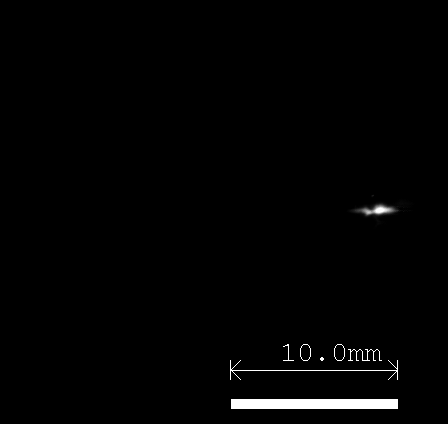
\includegraphics[width=\textwidth]{assets/4 experiments/V1 Spark Ignition Frames/LSP142_SPRK15_Fr32.bmp}
        \caption{\qty{3.2}{ms}}
        %\label{fig:V1_ignition_frames_16}
    \end{subfigure}
    \hfill
    \begin{subfigure}[t]{0.3\textwidth}
        \centering
        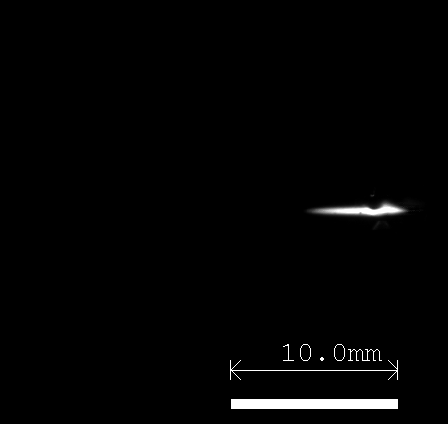
\includegraphics[width=\textwidth]{assets/4 experiments/V1 Spark Ignition Frames/LSP142_SPRK15_Fr33.bmp}
        \caption{\qty{3.3}{ms}}
        %\label{fig:ignition_frames_17}
    \end{subfigure}
    \hfill
    \begin{subfigure}[t]{0.3\textwidth}
        \centering
        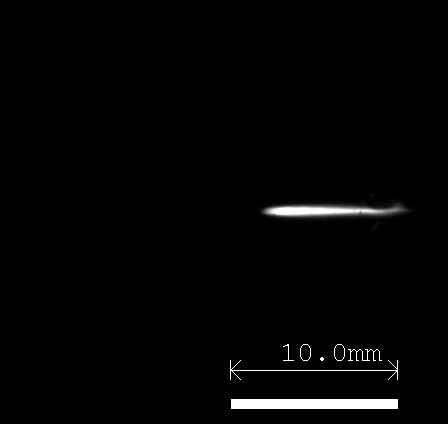
\includegraphics[width=\textwidth]{assets/4 experiments/V1 Spark Ignition Frames/LSP142_SPRK15_Fr35.bmp}
        \caption{\qty{3.5}{ms}}
        %\label{fig:ignition_frames_18}
    \end{subfigure}
    \begin{subfigure}[t]{0.3\textwidth}
        \centering
        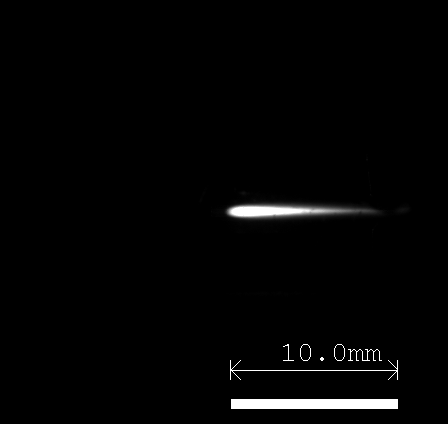
\includegraphics[width=\textwidth]{assets/4 experiments/V1 Spark Ignition Frames/LSP142_SPRK15_Fr38.bmp}
        \caption{\qty{3.8}{ms}}
        %\label{fig:ignition_frames_19}
    \end{subfigure}
    \hfill
    \begin{subfigure}[t]{0.3\textwidth}
        \centering
        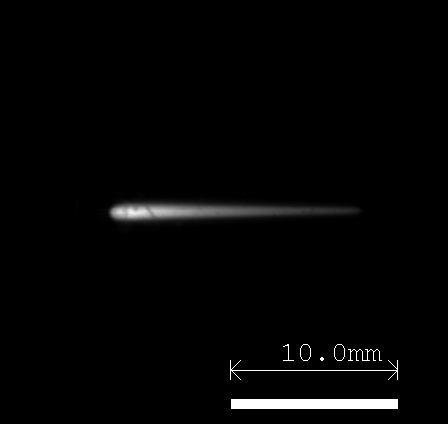
\includegraphics[width=\textwidth]{assets/4 experiments/V1 Spark Ignition Frames/LSP142_SPRK15_Fr69.bmp}
        \caption{\qty{6.9}{ms}}
        %\label{fig:ignition_frames_20}
    \end{subfigure}
    \hfill
    \begin{subfigure}[t]{0.3\textwidth}
        \centering
        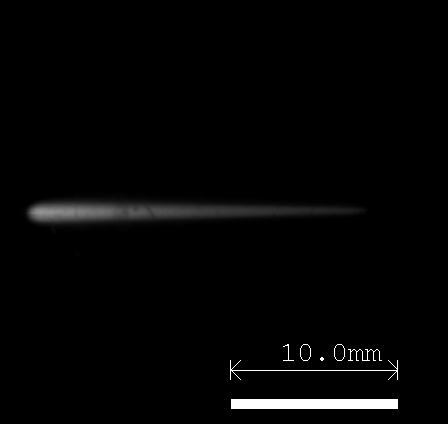
\includegraphics[width=\textwidth]{assets/4 experiments/V1 Spark Ignition Frames/LSP142_SPRK15_Fr130.bmp}
        \caption{\qty{13.0}{ms}}
        %\label{fig:ignition_frames_21}
    \end{subfigure}
    \caption{LSP spark initiation: \qty{3080}{W}, \qty{20}{bar}. \shotsettings{LSP142\_SPRK15}{0.1?? CHANGE}{22}{2048}}
    \label{fig:V1_spark_initiation_frames}
\end{figure}

        Selected frames\comment[id=BZ]{(...) pulse not exactly 10 ms or what?} of an entire LSP lifetime are shown in \autoref{fig:growth_frames}\comment[id=ED]{Starts at 1.6~ms, ends at 11.6~ms, \emph{ergo} 10~ms}. The initially rapid LSP growth ($\sim$\qty{9}{m.s^{-1}}) slows down as it approaches steady conditions, with the front speed decreasing to less than \qty{1}{m.s^{-1}} by the end of the laser pulse. \deleted{Steady-state conditions have thus not been truly achieved with full-power, 10 ms pulses.}The LSP responded practically instantaneously to the end of the laser pulse, as it dissipated from the high speed footage in the span of 1--2 frames \added{(0.1--0.2~ms)}. 

            \added{The fact that the plasma was still growing, albeit slowly, at the end of the laser pulse suggests that true steady-state conditions for the plasma are not yet attained within full-power 10-ms pulses. Unfortunately, the available equipment provided few metrics to quantify the (un)steadiness of flow and plasma conditions within the short time of a laser pulse. Spectroscopy measurements, which could potentially provide a time-dependent measure of plasma temperatures, required a minimum integration time of \qty{3.8}{ms}, allowing for \emph{at most} three measurements (only one was taken per pulse for this project). Time-dependent laser absorption and pressure measurements would require CW operation. This only left changes in the appearance of the LSP seen in high-speed footage as means to determine steady conditions.}

            \added{Nevertheless, the rates of change in the size and brightness of the LSP by the end of the pulse are significantly slower than those at plasma ignition. Furthermore, tests using stepped-pulse profiles discussed in \autoref{sec:results_powerthreshold} show a stable plasma appearance after readjusting to a sudden drop in laser power. Although possible, it seems unlikely the plasma conditions would drastically change over a timescale orders of magnitude greater than that of its readjustment, which appears to take place in a few \unit{ms}.}

            \added{Attempts were made at operating the experiment in a periodic or quasi-steady state by sending repeated laser pulses after a successful ignition. If a sufficient number of free electrons were still present after the extinction of the LSP, these residual electrons could perhaps allow for a subsequent LSP ignition without the use of an igniter. Tests were performed by sending full-power 10-ms pulses at the laser's maximum duty cycle of 10\%, but no re-ignition was observed. The laser's duty cycle created \qty{90}{ms} gaps in laser irradiation, enough time for the argon to dissipate its heat.}
            
            \begin{figure}[h]
    \centering
    \begin{subfigure}[t]{0.47\textwidth}
        \centering
        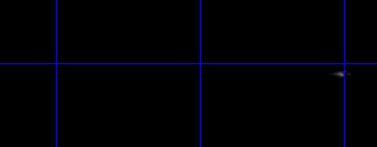
\includegraphics[width=\textwidth]{assets/5 results/1msFrames/16.jpg}
        \caption{\qty{1.6}{ms}}
        \label{fig:growth_frames_16}
    \end{subfigure}
    \hfill
    \begin{subfigure}[t]{0.47\textwidth}
        \centering
        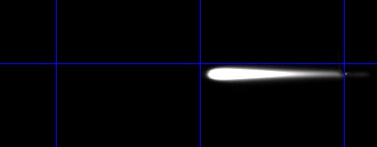
\includegraphics[width=\textwidth]{assets/5 results/1msFrames/26.jpg}
        \caption{\qty{2.6}{ms}}
        \label{fig:growth_frames_26}
    \end{subfigure}
    \hfill
    \begin{subfigure}[t]{0.47\textwidth}
        \centering
        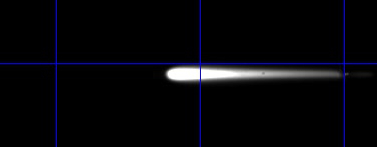
\includegraphics[width=\textwidth]{assets/5 results/1msFrames/36.jpg}
        \caption{\qty{3.6}{ms}}
        \label{fig:growth_frames_36}
    \end{subfigure}
    \hfill
    \begin{subfigure}[t]{0.47\textwidth}
        \centering
        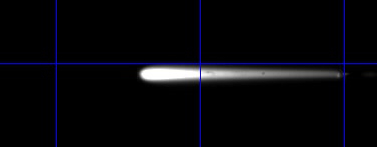
\includegraphics[width=\textwidth]{assets/5 results/1msFrames/46.jpg}
        \caption{\qty{4.6}{ms}}
        \label{fig:growth_frames_46}
    \end{subfigure}
    \hfill
    \begin{subfigure}[t]{0.47\textwidth}
        \centering
        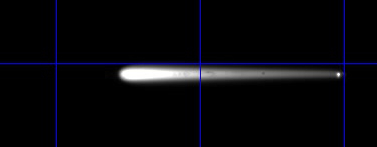
\includegraphics[width=\textwidth]{assets/5 results/1msFrames/56.jpg}
        \caption{\qty{5.6}{ms}}
        \label{fig:growth_frames_56}
    \end{subfigure}
    \hfill
    \begin{subfigure}[t]{0.47\textwidth}
        \centering
        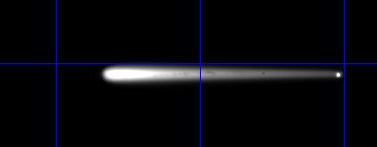
\includegraphics[width=\textwidth]{assets/5 results/1msFrames/66.jpg}
        \caption{\qty{6.6}{ms}}
        \label{fig:growth_frames_66}
    \end{subfigure}
    \hfill
    \begin{subfigure}[t]{0.47\textwidth}
        \centering
        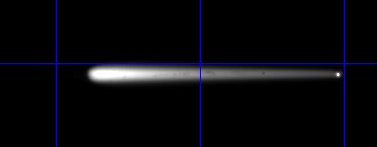
\includegraphics[width=\textwidth]{assets/5 results/1msFrames/76.jpg}
        \caption{\qty{7.6}{ms}}
        \label{fig:growth_frames_76}
    \end{subfigure}
    \hfill
    \begin{subfigure}[t]{0.47\textwidth}
        \centering
        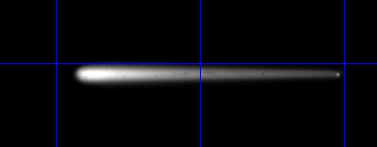
\includegraphics[width=\textwidth]{assets/5 results/1msFrames/86.jpg}
        \caption{\qty{8.6}{ms}}
        \label{fig:growth_frames_86}
    \end{subfigure}
    \hfill
    \begin{subfigure}[t]{0.47\textwidth}
        \centering
        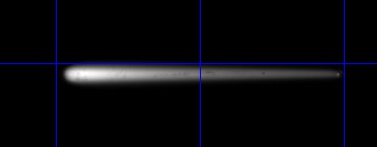
\includegraphics[width=\textwidth]{assets/5 results/1msFrames/96.jpg}
        \caption{\qty{9.6}{ms}}
        \label{fig:growth_frames_96}
    \end{subfigure}
    \hfill
    \begin{subfigure}[t]{0.47\textwidth}
        \centering
        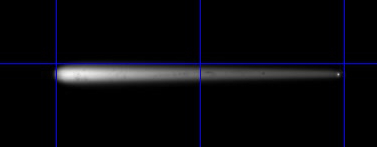
\includegraphics[width=\textwidth]{assets/5 results/1msFrames/106.jpg}
        \caption{\qty{10.6}{ms}}
        \label{fig:growth_frames_106}
    \end{subfigure}
    \hfill
    \begin{subfigure}[t]{0.47\textwidth}
        \centering
        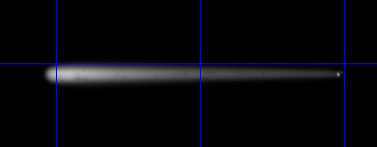
\includegraphics[width=\textwidth]{assets/5 results/1msFrames/116.jpg}
        \caption{\qty{11.6}{ms}}
        \label{fig:growth_frames_116}
    \end{subfigure}
    \caption[LSP growth throughout 10-ms-laser pulse]{LSP growth throughout 10-ms-laser pulse: \qty{3080}{W}, \qty{20.29}{bar}. The blue grid is spaced by \qty{10}{mm}. \shotsettings{LSP1\_PS1}{0.1}{22}{2048}}
    \label{fig:growth_frames}
\end{figure}

    \clearpage
    \section{Power threshold} \label{sec:results_powerthreshold}
        Once LSP ignition had been confirmed, work began on reproducing power threshold experiments, a frequent topic in LSP research. The aim of this experiment is to determine the minimum laser power required to sustain a steady plasma, at a given pressure. Knowing this power threshold is useful to establish the operation bounds of an LSP facility, whether it is a laboratory experiment or a laser-thermal thruster. Several of such experiments have been performed for argon with fiber-lasers: the work of \textcite{zimakovInteractionNearIRLaser2016, matsuiGeneratingConditionsArgon2019,luCharacteristicDiagnosticsLaserStabilized2022} will thus be used for comparison.
        
        \subsection{Methodology}
            The test section would be pressurized with argon to a desired pressure between 3 and 20~bar. Then, determining the power threshold was done through a process akin to a binary search or bisection root-finding algorithm in computer science: LSP would be ignited first at the maximum setpoint power to confirm that the laser and igniter were aligned such that LSP was achievable. Power would then be reduced to a point far below the threshold (10\% power) to confirm that LSP was not achieved. This brackets the threshold point. Subsequent tests would be performed at a power setpoint in the middle of this iteratively shrinking bracket, until the threshold was determined to be within approximately \qty{50}{W} below the last successful LSP test.

            This series of tests were performed with both spark and wire ignition. One issue encountered with wire ignition was that while lower laser powers could theoretically sustain LSP, they would not necessarily be sufficient to ignite it. \added{Low laser powers may not raise the temperature of the wire at the ignition point fast enough to trigger thermionic emission, as discussed in \autoref{subsec:results_wireignition}, as heat would be conducted away from the laser focal point. No successful ignition was observed below \qty{1}{kW} of laser power.}
            
            To circumvent this issue, stepped laser pulse profiles were used instead of constant laser power. An example of such a pulse is shown in \autoref{fig:pulse_stepProfile}: the pulse begins at 100\% setpoint power for \qty{0.5}{ms} to initiate the LSP off of the tungsten wire. The power would then be stepped down to the desired power level, which would be maintained for as long as possible to ensure that the LSP could re-adjust to steady conditions.

            \begin{figure}[h]
                \centering
                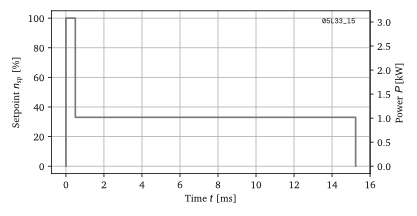
\includegraphics[]{assets/5 results/pulse_profile}
                \caption[Typical stepped-pulse profile: \texttt{05L33\_15}]{Typical stepped-pulse profile: \texttt{05L33\_15}. A complete list of stepped-pulse specifications can be found in \autoref{chp:app_pulseShapes}.}
                \label{fig:pulse_stepProfile}
            \end{figure}

            Whether LSP could be considered steady for a given test was determined by observing its behavior in the high-speed footage. It needed to fulfill two conditions:
            \begin{enumerate}
                \item The LSP is still visible at the end of the laser pulse
                \item The LSP is not visibly changing by the time the laser pulse ended, i.e., it is not shrinking or dimming significantly.
            \end{enumerate}
            As plasma brightness changed with laser power, the variable ND filter would be adjusted to determine whether a vanishing plasma was unstable or simply too dim to be picked up through the lens filters.



        \subsection{Results}
            The resulting power threshold plot can be seen in \autoref{fig:powerthreshold}. Both spark and wire ignition experiments are shown, along with data reported by \textcite{zimakovInteractionNearIRLaser2016,matsuiGeneratingConditionsArgon2019,luCharacteristicDiagnosticsLaserStabilized2022}. The use of wire ignition shows a significant improvement in the minimum power required to sustain LSP over the spark-ignition method. The improved reliability and ease of alignment afforded by wire ignition enabled sustaining LSP down to hundreds of Watts, whereas spark ignition struggled to ignite and sustain LSP below \qty{1}{kW}. Note that the uncertainties indicated on the wire ignition data reflect the possible range in which the true power threshold lies and is not related to an uncertainty in the power measurement. \textcite{zimakovInteractionNearIRLaser2016} presented a model based on balancing input power with heat conduction ($P_\mathrm{h}$) and radiative losses ($P_\mathrm{r}$) under steady conditions, to evaluate the power threshold as a function of pressure $P_\mathrm{t}$. This expression is reproduced here as \autoref{eq:zimakov_threshold}:
            \begin{equation} \label{eq:zimakov_threshold}
                P_\mathrm{t} = P_\mathrm{h} + P_\mathrm{r}
            \end{equation}
            \citeauthor{zimakovInteractionNearIRLaser2016}'s experiments had experimentally estimated the parameters of this equation for argon as $p^2P_\mathrm{h} =$~\qty{26}{bar^2.kW} and $P_\mathrm{r} =$~\qty{240}{W}. This same model was fitted to this study's wire-ignited LSP data, yielding the following power threshold parameters: $p^2P_\mathrm{h} =$~\qty{11}{bar^2.kW} and $P_\mathrm{r} =$~\qty{178}{W}. These values can be interpreted, respectively, as the minimum laser power to sustain LSP at \qty{1}{bar}, and the limiting laser power under which no LSP can be sustained even at high pressures. \added{This relation only holds in the steady case---transient conditions would result in an unbalance of \autoref{eq:zimakov_threshold}. For instance, a supplied laser power above the threshold power would deposit more heat in the LSP than it could dissipate by conduction and radiation. This would likely result in the growth of the plasma core to increase the strength of both of its heat dissipation mechanisms.}

            \added{The experimental data suggests that the threshold power required to sustain plasma beyond \qty{10}{bar} is lower than the nominal average power of the laser used in this project, i.e., \qty{300}{W}. This would imply that continuous operation of the LSP generator is possible at pressures of \qty{10}{bar} and above. Attempts were made to achieve continuous operation at the maximum rated pressure of the test section of \qty{20}{bar}, but neither spark nor wire ignition was successful. In the case of spark ignition, many of the issues discussed in \autoref{subsec:results_sparkignition} may have contributed to a failure to ignite. This could have been mitigated by configuring the spark igniter for repeated sparks, but this was not attempted. In the case of wire ignition, \qty{300}{W} is likely not sufficient to locally heat the wire to thermionic-emission temperatures before heat is conducted away from the laser-irradiated point. Stepped-pulse profiles were used to circumvent this issue for power-threshold experiments, but the laser was not capable of emitting a stepped-pulse then transition to CW mode without interrupting emission. Continuous LSP operation could thus not be achieved with the stepped-pulse workaround.}

            \added{Considering that true steady plasma conditions may not have been attained in some cases, it should be noted that the experimentally determined power threshold may be lower than that of continuous LSP operation. The short pulse duration combined with the high ignition power may allow the LSP to remain stable for the duration of the pulse when it may not have done so over a longer timescale, i.e., over several seconds. Further experiments in CW mode should be performed to provide definite power threshold data.}

            The discrepancy in the power thresholds achieved across different experiments is due in part to the optical quality of the focused beam, as suggested by \textcite{luCharacteristicDiagnosticsLaserStabilized2022}, who have so far achieved the lowest power-threshold results for fiber-laser-sustained argon plasma. As the literature data is all from spark-ignited experiments, direct comparisons to wire-ignition tests may be limited. However, this suggests that a low power threshold can be readily achieved by a basic optical train and a simple wire-ignition system combined with stepped pulse profiles, competing with methodologies that require far greater precision and optical quality. 

            Qualitative observations were made on the LSP's response to the step-down in laser power. As seen in \autoref{fig:lsp_stepdown}, the decrease in input power is immediately apparent, with the plasma shrinking and dimming as soon as the power is dropped. The LSP re-adjusts to new power conditions in less than a millisecond. In this particular case, the LSP remained stable until the end of the laser pulse, \qty{14.8}{ms} after the step-down in power.


            \begin{figure}[h]
                \centering
                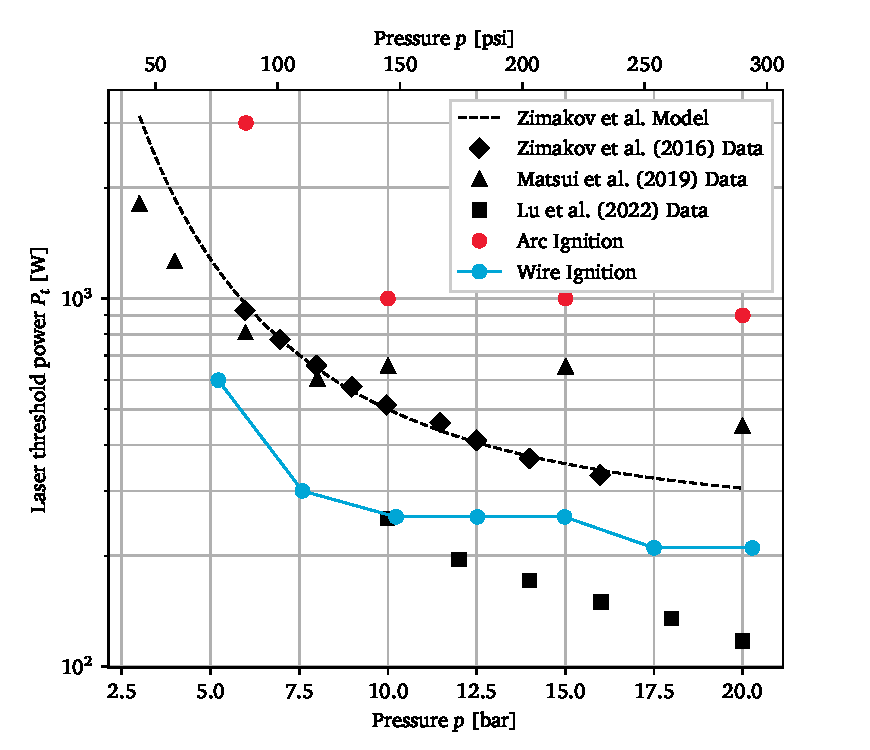
\includegraphics[]{assets/5 results/powerthreshold}
                \caption[Pressure-Power LSP threshold exploration]{Pressure-Power LSP threshold exploration. \textcite{zimakovInteractionNearIRLaser2016}'s model is fitted to wire-ignition data as the blue dashed line.}
                \label{fig:powerthreshold}
            \end{figure}

            \begin{figure}[h]
                \centering
                \begin{subfigure}[t]{0.32\textwidth}
                    \centering
                    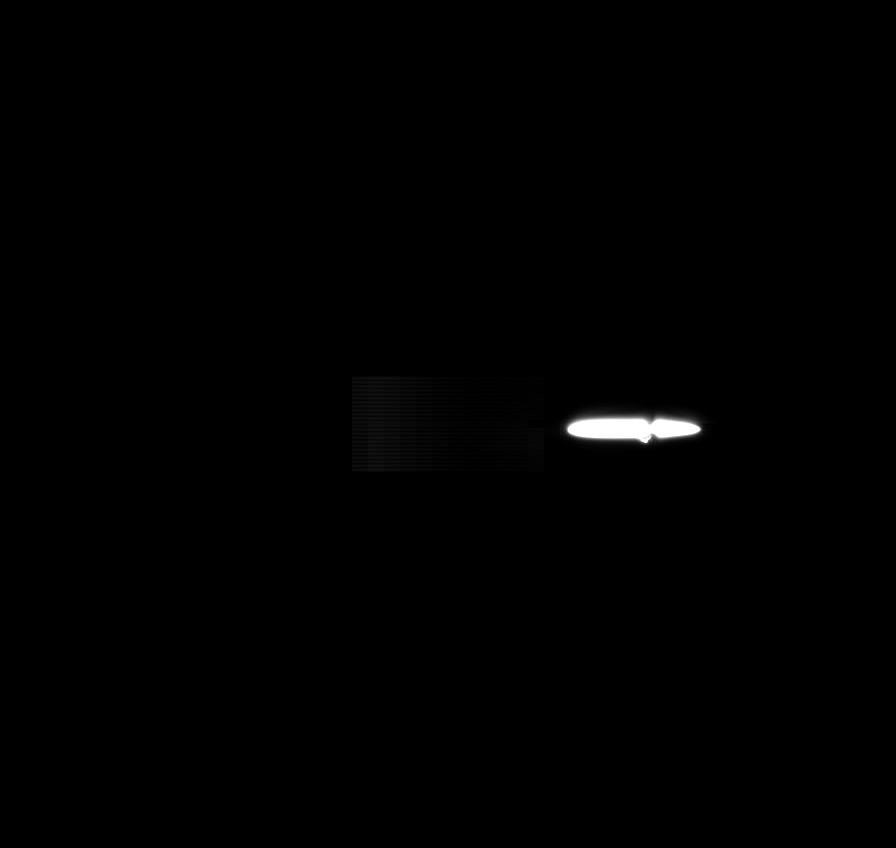
\includegraphics[trim=7.6in 5.3in 2.4in 5.5in, clip, width=\textwidth]{assets/5 results/LSP34_PS28/20.jpg}
                    \caption{\qty{2.0}{ms}, before step-down}
                    \label{fig:lsp_stepdown_20}
                \end{subfigure}
                \hfill
                \begin{subfigure}[t]{0.32\textwidth}
                    \centering
                    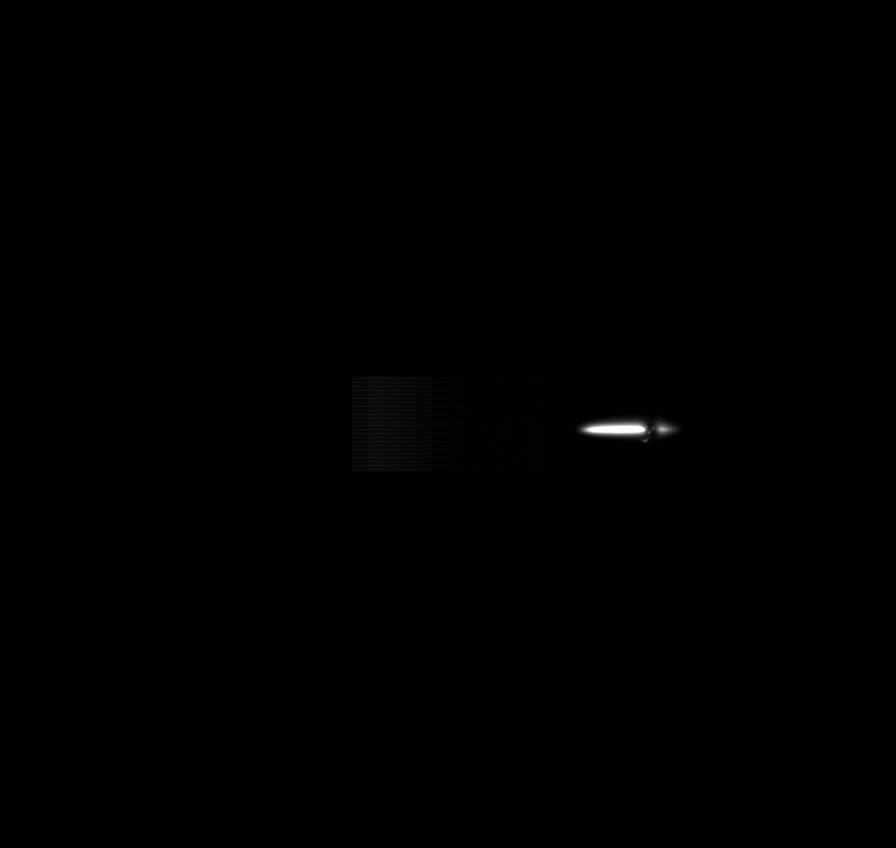
\includegraphics[trim=7.6in 5.3in 2.4in 5.5in, clip, width=\textwidth]{assets/5 results/LSP34_PS28/21.jpg}
                    \caption{\qty{2.1}{ms}, after step-down}
                    \label{fig:lsp_stepdown_21}
                \end{subfigure}
                \hfill
                \begin{subfigure}[t]{0.32\textwidth}
                    \centering
                    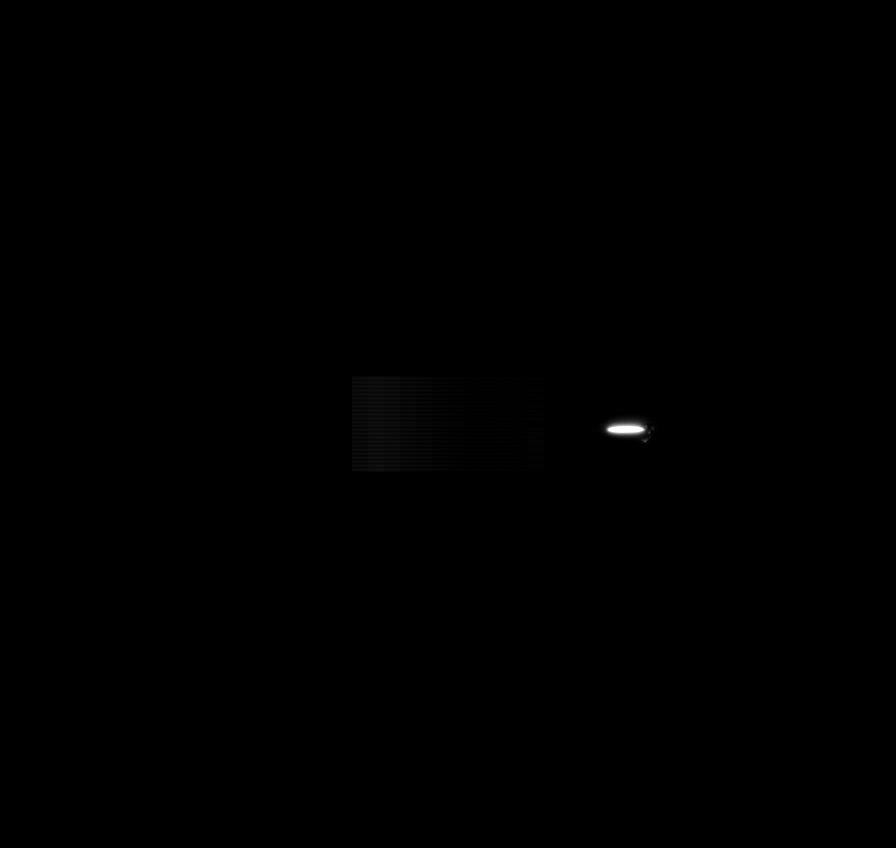
\includegraphics[trim=7.6in 5.3in 2.4in 5.5in, clip, width=\textwidth]{assets/5 results/LSP34_PS28/28.jpg}
                    \caption{\qty{2.8}{ms}, steady-state}
                    \label{fig:lsp_stepdown_28}
                \end{subfigure}
                \caption[LSP adjusting to step-down in power]{LSP adjusting to step-down in power, from 100\% to 8.5\% (\qty{255}{W}). \shotsettings{LSP34\_PS28}{0.1}{4}{2048}, pulse profile: \texttt{05L8.5\_15}, pressure: \qty{10.23}{bar}}
                \label{fig:lsp_stepdown}
            \end{figure}

    \clearpage
    \section{Laser Absorption} \label{sec:exp_absorption}
        Despite the reliability issues of spark ignition, LSP absorption data was successfully acquired at various pressures and laser pulse energies. Incomplete absorption of the incident laser radiation by IB is one of the major sources of inefficient heat deposition, so quantifying this loss is important to control it, reduce it, and  eventually optimize an LTP thruster.
        
        \subsection{Methodology}
            The Gentec power meter recorded the incident pulse energy for a subset of spark-ignited LSPs. Unfortunately, due to this ignition system's reliability issues, discussed in \autoref{sec:ignitiontest}, a systematic exploration of the variation in absorption due to experimental parameters could not be performed. Nevertheless, some preliminary data was acquired, with some consistency observed at \qty{20}{bar} of pressure.

            Constant-power, \num{10}-\unit{ms} laser pulses were focused into the test section to ignite LSP. As seen in \autoref{tab:expTimeline}, a buffer time of \qty{1}{ms} between the start of the pulse and the spark ignition was used to ensure that the spark was triggered while the laser was on. The laser absorption $a$ by the LSP was defined as follows:
            \begin{equation}
                a = 1-\frac{E_\tau}{E_\mathrm{in}}
            \end{equation}
            Where $E_\tau$ is the measured (transmitted) energy reaching the power meter and $E_\mathrm{in}$ is the pulse energy incident on the LSP. Both variables were determined by correcting both for the losses through the experiment optics (given in \autoref{tab:opticalLoss}) and the \num{1}-\unit{ms} buffer time. \added{The laser absorption constitutes one component of the heat deposition efficency studied in \autoref{sec:heate_deposition}.}

        \subsection{Results}
            Calculated LSP absorption is tabulated in \autoref{tab:LSP_absorption}. Although there are a few outliers, overall absorption appears to lie between 70\% and 90\%. This is visualized in \autoref{fig:absorption_ap}. Data for several tests performed at a nominal pressure of \qty{20}{bar} can be seen in \autoref{fig:absorption_20bar}, where a linear function was fitted to the data to determine an average absorption factor of 79\%.

            \begin{table}[h]
\centering
\caption[LSP energy absorption data]{LSP energy absorption data. $p$ is the nominal pressure; $E_\mathrm{pulse}$, $E_\mathrm{in}$, $E_\tau$, and $E_a$ are the laser pulse energy, input energy, transmitted energy, and computed absorption of the LSP, respectively.}
\label{tab:LSP_absorption}
\begin{tabular}{@{}lrrrrr@{}}
\toprule
Shot ID & $p$ [bar] & $E_\mathrm{pulse}$ [J] & $E_\mathrm{in}$ [J] & $E_\tau$ [J] & $a$ [-] \\
\midrule
\verb|LSP210_SPX11| &     20.20 &                  30.80 &               27.56 &         5.81 &    0.79 \\
\verb|LSP211_SPX12| &     20.00 &                  30.80 &               27.56 &         6.16 &    0.78 \\
\verb|LSP212_SPX13| &     20.00 &                  18.48 &               16.53 &         4.95 &    0.70 \\
\verb|LSP213_SPX14| &     19.90 &                  12.32 &               11.02 &         1.41 &    0.87 \\
\verb|LSP215_SPX16| &     20.00 &                  30.80 &               27.56 &         5.15 &    0.81 \\
\verb|LSP216_SPX17| &      6.09 &                  30.80 &               27.56 &         8.62 &    0.69 \\
\verb|LSP217_SPX18| &     10.10 &                  20.54 &               18.38 &        14.80 &    0.19 \\
\verb|LSP219_SPX20| &     15.00 &                  10.16 &                9.09 &         7.83 &    0.14 \\
\bottomrule
\end{tabular}
\end{table}

            
            \begin{figure}[h]
                \centering
                \begin{subfigure}[t]{0.47\textwidth}
                    \centering
                    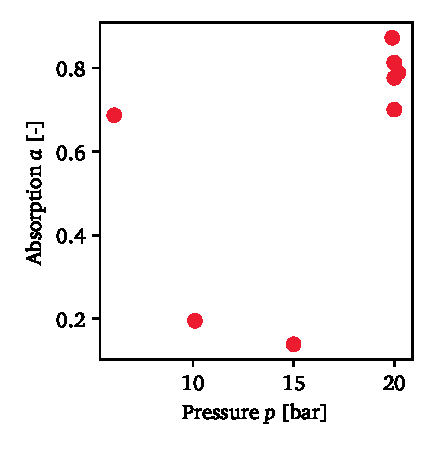
\includegraphics[width=\textwidth]{assets/5 results/absorption_ia}
                    \caption{Absorption across a range of pressure. Variable pulse energy and chamber pressure.}
                    \label{fig:absorption_ap}
                \end{subfigure}
                \hfill
                \begin{subfigure}[t]{0.47\textwidth}
                    \centering
                    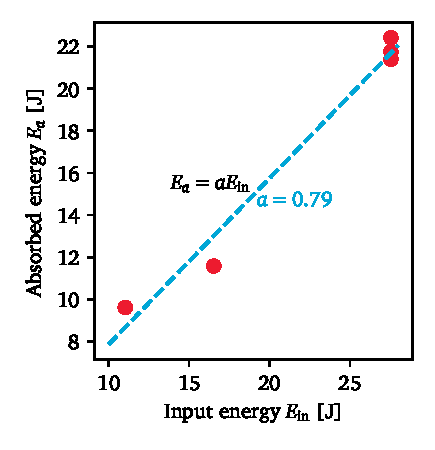
\includegraphics[width=\textwidth]{assets/5 results/absorption_20bar}
                    \caption{Input energy vs. absorbed energy, calculation of absorption}
                    \label{fig:absorption_20bar}
                \end{subfigure}
                \caption{Estimated energy absorption of LSP, \qty{20}{bar}}
                \label{fig:LSP_absorption_data}
            \end{figure}

            Such absorption figures appear to be in agreement with LSP literature stating that most of the laser radiation can be absorbed by the LSP under the right conditions (\textcite{keeferLaserSustainedPlasmas1989}). However, much higher absorption was shown to be achievable under some conditions, such as forced convection (\textcite{fowlerIgnitionMaintenanceSubsonic1975}). For instance, experiments by \textcite{toyodaThrustPerformanceCW2002} show between 80\% and 99\% absorption depending on the working gas and experimental conditions.

            This absorption data can also be paired with LSP footage to approximate the absorption coefficient of the LSP. For instance, \autoref{fig:LSP205_SPX6} shows the length measurement of an LSP (\qty{10}{bar}, \qty{3080}{W}) to be \qty{22}{mm} at its fullest extent.

            \begin{figure}[h]
                \centering
                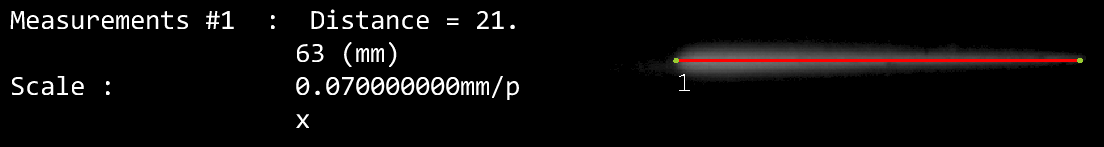
\includegraphics[width=\textwidth]{assets/5 results/LSP6_10.23_length.png}
                \caption[Length estimation of LSP]{Length estimation of LSP. \qty{10.23}{bar}, \num{30.8}-\unit{J} pulse. \shotsettings{LSP205\_SPX6}{0.1}{11}{2048}}
                \label{fig:LSP205_SPX6}
            \end{figure}

            Considering the transmission of radiation through an absorbing medium using the Beer-Lambert law:
            \begin{equation} \label{eq:beerlambert}
                \frac{I(d)}{I_0} = e^{-\alpha d}
            \end{equation}
            By considering the energy transmission $E_\tau/E_\mathrm{in}$ to be equivalent to the left-hand side of \autoref{eq:beerlambert}, and approximating the path length $d$ as the LSP length, the absorption coefficient can be estimated as follows:
            \begin{equation}
                \alpha = \frac{\ln{(E_\tau/E_\mathrm{in})}}{-d}
            \end{equation}
            For \texttt{LSP205\_SPX6}, this evaluates to \qty{73}{m^{-1}}. This in fact appears to match the absorption coefficient calculations performed in \autoref{chp:models}. \autoref{fig:ib_coeff} predicts an absorption coefficient of \qty{67}{m^{-1}}, while the calculations of \textcite{matsuiGeneratingConditionsArgon2019} predict a value of \qty{58}{m^{-1}}. While not in perfect agreement with theory, this estimate does appear to provide a value on the same order as predicted by IB absorption models.

            As mentioned earlier, the reliability issues of the spark-ignition system prevented the systematic study of LSP absorption characteristics. The $\alpha$ estimate above unfortunately cannot account for the changing absorption/transmission as the LSP grows and assumes a path length based on the final LSP size. Performing absorption measurements under CW regime would improve the measure of $\alpha$ considerably, as measurements could be made once the LSP is fully developed and steady.

    \section{Heat deposition} \label{sec:heate_deposition}
        To fulfill this project's second research objective, i.e., determining LSP heat deposition in the working gas, the change in pressure from initial conditions was monitored with a PCB Piezotronics pressure transducer. As discussed on page \pageref{sec:design_pressuresensor}, this would theoretically allow the estimation of heat deposition without the need to directly track the temperature of the gas, which would have been a major challenge for a millisecond-scale event.

        \subsection{Methodology}
            The pressure data was collected in parallel with other experiments, all ignited using a wire-ignition method. As seen in \autoref{fig:finalsetup_static}, the pressure transducer was integrated using an instrumentation plug on top of the test section, \qty{1.5}{in} downstream from the ignition point. The transducer's signal was then processed by a signal conditioner whose output was recorded on an oscilloscope, along with the laser's internal power meter reading. This allowed the synchronization of both the laser's power and the pressure in the test section.

            A sample pressure signal is provided in \autoref{fig:pressure_noise}. The oscilloscope data featured significant noise, which was filtered out with an infinite impulse response filter to facilitate analysis. Pressure data was acquired for a variety of initial pressures and laser power levels.

            \begin{figure}[h]
                \centering
                \begin{subfigure}[t]{0.47\textwidth}
                    \centering
                    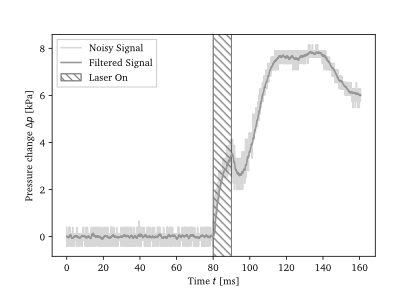
\includegraphics[width=\textwidth]{assets/5 results/pressure_noise}
                    \caption{Typical pressure change during and after LSP at \qty{3080}{W}, \qty{20.29}{bar}}
                    \label{fig:pressure_noise}
                \end{subfigure}
                \hfill
                \begin{subfigure}[t]{0.47\textwidth}
                    \centering
                    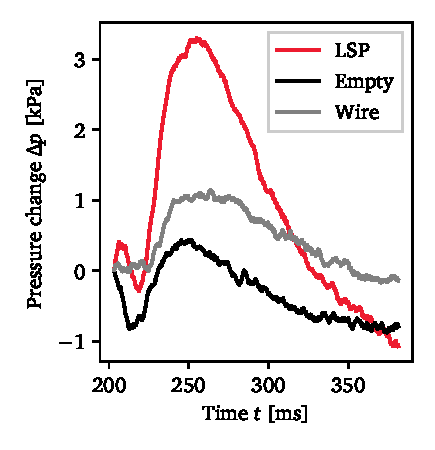
\includegraphics[width=\textwidth]{assets/5 results/pressure_elim}
                    \caption{Pressure rise due to alternate heat transfer mechanisms}
                    \label{fig:pressure_elim}
                \end{subfigure}
                \caption{Denoising of pressure data and comparison to other sources of heat}
            \end{figure}

            
            To ensure that the resulting pressure rise was primarily caused by the LSP, two tests were performed to rule out the effects of other potential factors:
            \begin{enumerate}
                \item The laser directly incident on the test section walls could heat up the walls which would then heat up the gas
                \item The ignition wire heating up could transfer its heat to the surrounding gas.
            \end{enumerate}
            While either scenario does ultimately heat up the gas, neither mechanism reflects the ideal operation of a laser-thermal thruster, where the plasma itself should be the dominant heat source. To quantify these effects, the following tests were performed at an initial pressure of \qty{10}{bar} and the resulting pressure rise was recorded:
            \begin{enumerate}
                \item The laser (\qty{10}{ms}, 100\%) was pointed into an empty test section, such that the laser would be directly incident on an opaque backplate.
                \item A constant 20\%, \num{19.8}-\unit{ms} pulse (equivalent in energy to a \texttt{1L20\_15} stepped pulse yet insufficient for ignition) was focused on the ignition wire.
            \end{enumerate}
            The pressure rise of these tests\comment[id=BZ]{Why is pressure rise so limited? Would this lead to recommendations for adaptations to the test facility if you would redo this research again?}\comment[id=ED]{This is now addressed in the Further work section} was then compared to that of a successful LSP at \qty{10}{bar}, sustained with a \texttt{1L20\_15} stepped pulse (\qty{12.1}{J}). This is shown in \autoref{fig:pressure_elim}. Some measurable effect on pressure is detected from both of these mechanisms, however, the pressure rise from LSP is greater by a factor of three compared to direct heating of the ignition wire. Furthermore, the tests mentioned above represent an absolute worst-case scenario for the magnitude of these heat transfer mechanisms. Absorption measurements discussed in \autoref{sec:exp_absorption} show that the majority of the laser power is absorbed by the LSP. This leaves less power for heat transfer by wire or chamber wall heating. Heating via the chamber walls in particular is not expected to significantly contribute to overall heat transfer, as the ignition wire would absorb most of any laser power transmitted through the LSP, and direct irradiation had only a minor effect in the first place.

        \subsection{Results}
            The pressure rise seen in \autoref{fig:pressure_noise} exhibits features that were consistently observed at different initial pressures and different laser powers. Namely, the pressure appears to rise continuously while the laser and the LSP is active. As soon as the laser is off and the LSP is extinguished, a small drop in pressure is observed, which is then followed by another, higher rise in pressure. Once the pressure reaches a maximum, usually around \qty{40}{ms} after the end of the laser pulse, it decreases \replaced{progressively}{a at slower rate relative to the rise,} as the gas loses heat through conduction with the chamber walls. Such a pressure variation is unlikely to be from traveling pressure waves: The speed of sound in argon at \qty{20}{\degreeCelsius} is \qty{319}{mm.ms^{-1}}, i.e., the test section's length every millisecond, while the observed pressure variation occurs over several hundredths of a second. This suggests that the pressure change observed by the pressure transducer reflects that of the overall test section static pressure.

            \added{The continuing pressure rise while the laser (and LSP) is active would suggest that the test-section conditions are in a transient state---the pressure does not stabilize to some level. This is expected to some degree: \qty{10}{ms} is unlikely to be enough time for the working gas to reach steady conditions. Furthermore, as these tests are performed in a static mass of argon, the only mechanism to balance this pressure rise is heat transfer out of the test section. This is not expected to occur within that timescale, as the test section would have to heat up significantly to dissipate kW of laser power. In any case, this is not conflicting with the idea that the plasma is approaching/has reached steady conditions. The plasma could certainly reach a state where laser absorption is balanced out by heat dissipation long before the overall test-section conditions have reached steady-state.}

            \begin{figure}[h]
                \centering
                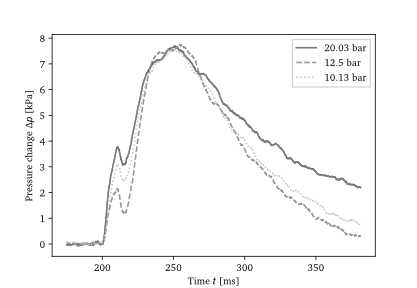
\includegraphics[]{assets/5 results/pressure_pressures}
                \caption{Effect of varying initial pressure on pressure rise resulting from LSP}
                \label{fig:pressure_pressures}
            \end{figure}

            \autoref{fig:pressure_pressures} shows the pressure variation for a range of initial nominal pressures. As mentioned earlier, the features of this pressure rise remain consistent with a local maximum reached at the end of the laser pulse (\qty{10}{ms}). The magnitude of the pressure change does not appear to be strongly affected by the initial pressure.\comment[id=ED]{Pressure rise calculation discussion moved to Chapter 4} \added{This consistent pressure profile could be explained as follows: the first rise in pressure appears to be directly linked with the lifetime of the LSP. The growth of the plasma occupies space in the test section at a lower density than the surrounding gas, and the sustained plasma dissipates heat into the test section. Both of these effects contribute to an increase in static pressure, and the change in the gradient of the pressure rise for lower-energy tests seems to support this: the sudden decrease in laser power during a stepped pulse coincides with slower LSP growth (or in some cases, stagnating or decreasing size) and a reduced pressure rise gradient on the pressure plots. This is seen in \autoref{fig:pressure_powers}. As the laser is turned off, the plasma immediately cools down and shrinks, allowing denser gas to occupy the LSP's volume, reducing the measured static pressure. This decrease is typically less pronounced for lower-energy tests, which would support this hypothesis. The heat remaining in the plasma core as it cools can no longer dissipate as effectively by radiation, and is thus distributed by convection throughout the test section, resulting in the second pressure rise.}
            % Assuming an even distribution of heat added into a closed system, the resulting pressure change $\Delta p$ can be expressed using the ideal gas equation and the change in temperature $\Delta T$ caused by a constant volume heat addition $Q_\mathrm{in}$:
            % \begin{gather*}
            %     \Delta pV = mR_\mathrm{g}\Delta T \\
            %     Q_\mathrm{in} = mc_V\Delta T \\
            %     \Delta p = \frac{R_\mathrm{g}Q_\mathrm{in}}{Vc_V}
            % \end{gather*}
            % \added{The specific heat at constant volume $c_V$ is taken to be that of room-temperature-and-pressure Argon: \qty{312}{J.kg^{-1}.K^{-1}}~\cite{lemmonThermophysicalPropertiesFluid2023}. }The resulting change in pressure is independent of the gas mass, and therefore, independent of the initial pressure for a set volume. This \added{initial-pressure independence }however \deleted{would} only hold\added{s} as long as the heat deposited in the gas $Q_\mathrm{in}$ is also independent on the initial pressure.


            \autoref{fig:pressure_powers} shows the effect of reducing the laser pulse energy on the resulting pressure rise. In this case, the peak pressure appears to be correlated with pulse energy, decreasing consistently with decreasing energy. Here again, the change from \qtyrange{20}{10}{bar} of initial pressure does not appear to have an effect on the resulting heat deposition. The intermediate peak in pressure appears to occur later for lower energy pulses, this is due in part to the longer pulse duration. Another feature of the lower energy pressure rises is a decrease in the rate of change of pressure during the pulse---there is a clear change as the pulse switched from the high setpoint for ignition, to the lower sustained setpoint.

            \begin{figure}[h]
                \centering
                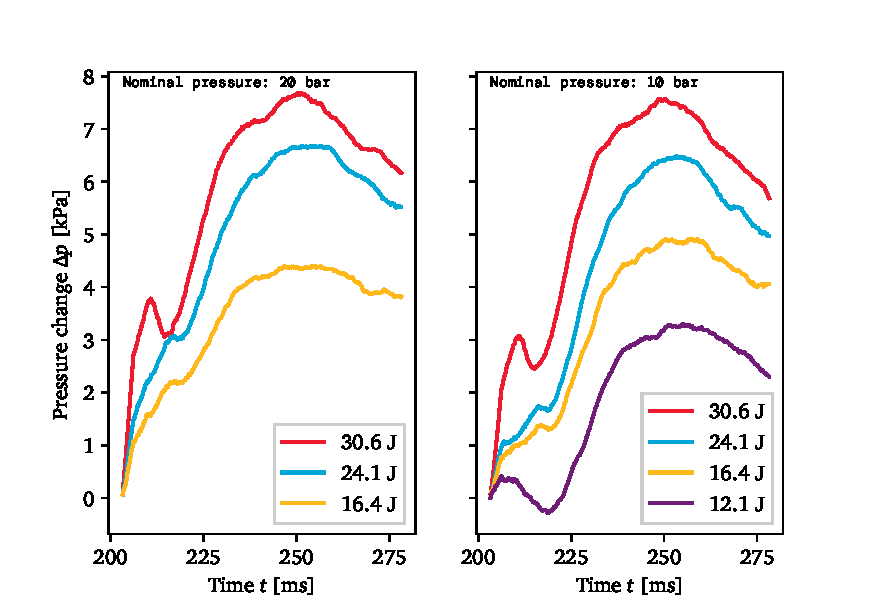
\includegraphics[]{assets/5 results/pressure_powers}
                \caption{Effect of varying laser pulse energy on pressure rise resulting from LSP}
                \label{fig:pressure_powers}
            \end{figure}

            A first estimation of the heat deposited in the working gas can be made based on the pressure change, assuming that the observed maximum pressure reflects a state where the heat has been distributed throughout the test section. 
            \begin{equation} \label{eq:heatdep}
                Q_\mathrm{in} = \frac{\Delta pVc_V}{R_\mathrm{g}}
            \end{equation}
            The heat-deposition efficiency $\eta$ can then be calculated as the ratio $Q_\mathrm{in}/E_\mathrm{in}$, which captures the overall efficiency of converting the incident laser power on the LSP into heat remaining in the propellant. This would include losses from incomplete laser absorption by the LSP, along with heat lost in the form of radiation, which would heat the chamber walls without really affecting the gas temperature. The detailed results of such a calculation are shown for a single LSP test in \autoref{fig:pressure_annotated}.

            \begin{figure}[h]
                \centering
                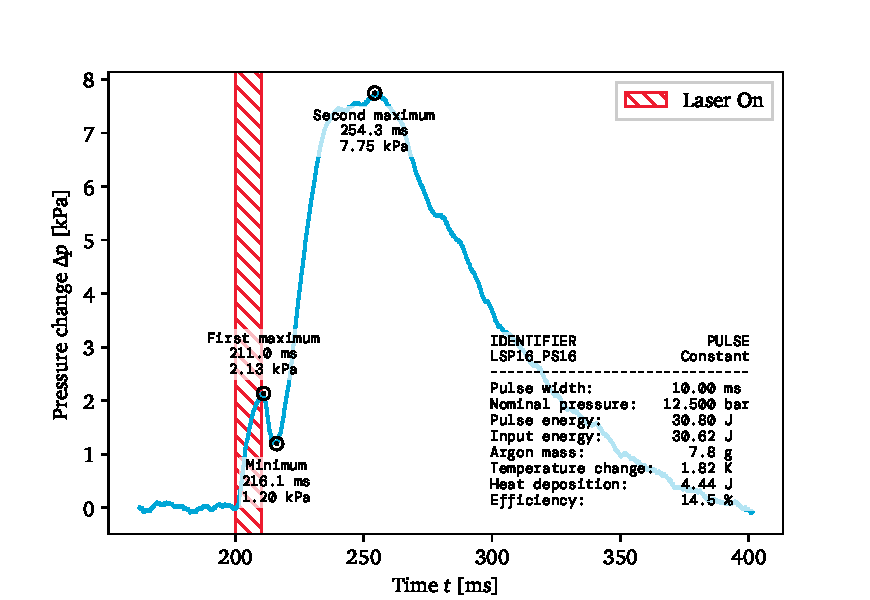
\includegraphics[]{assets/5 results/pressure_an_LSP16_PS16}
                \caption[Detailed analysis of pressure rise profile]{Detailed analysis of pressure rise profile, \qty{3080}{W}, \qty{12.5}{bar}.}
                \label{fig:pressure_annotated}
            \end{figure}


            Repeating this efficiency calculation for several LSPs sustained at various pressures and pulse energies yields \autoref{fig:heatEfficiency}. Heat-deposition efficiency is seen to be consistent at around 15\%, regardless of laser power or gas pressure. \added{This apparent independence of heat deposition efficiency could be explained if most of the heat in the LSP is dissipated by radiation. As mentioned in \autoref{chp:background}, argon does not have large absorption bands to capture the plasma's emitted radiation, whose continuum spectrum likely lies mostly in the near-UV bands based on Wien's law. Therefore, changing pressures would have little effect on the radiative heat absorption of the cooler surrounding gas and the plasma's radiated heat would be absorbed by the walls.}
            
            \added{Other studies have measured heat deposition efficiencies for LSP, usually using \ce{CO2}-laser-sustained plasmas. \textcite{chenEmissionSpectroscopyCw1989,mazumderSpectroscopicStudiesPlasma1987} have reported heat deposition efficiencies in flowing plasmas ranging from 35--62\%. This is significantly greater than the efficiency determined in this study. A possible factor for this discrepancy is the lack of flow in these static experiments. \textcite{chenEmissionSpectroscopyCw1989} report that greater flow speeds (2--10~\unit{m.s^{-1}}) improve heat deposition efficiencies. As mentioned in \autoref{sec:exp_absorption}, laser absorption by the LSP is one of the major components of the overall heat-deposition efficiency, implying that 20\% of the laser energy does not even enter the plasma. Of the 80\% that does get absorbed and turned into heat, 81\% of it is lost (i.e., 65\% of the laser energy), likely by radiation, to the test section walls. This distribution is illustrated in \autoref{fig:heatdep_sankey}.}

            \begin{figure}[h]
                \centering
                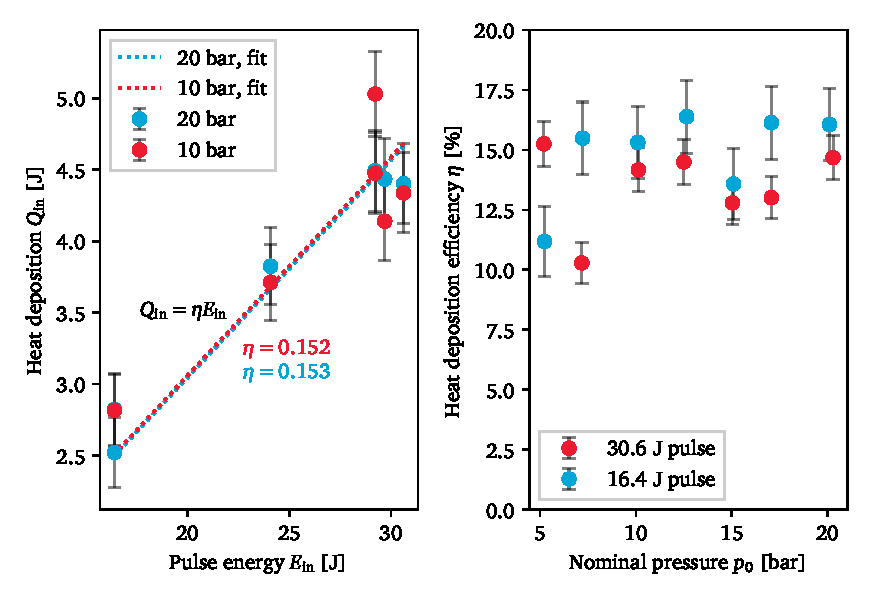
\includegraphics[]{assets/5 results/heatEfficiency}
                \caption[Heat-deposition efficiency of LSP]{Heat-deposition efficiency of LSP. Left: calculation at 20 and 10~bar; right: consistency across a range of pressures, for two different pulse energies}
                \label{fig:heatEfficiency}
            \end{figure}

            \begin{figure}[h]
                \centering
                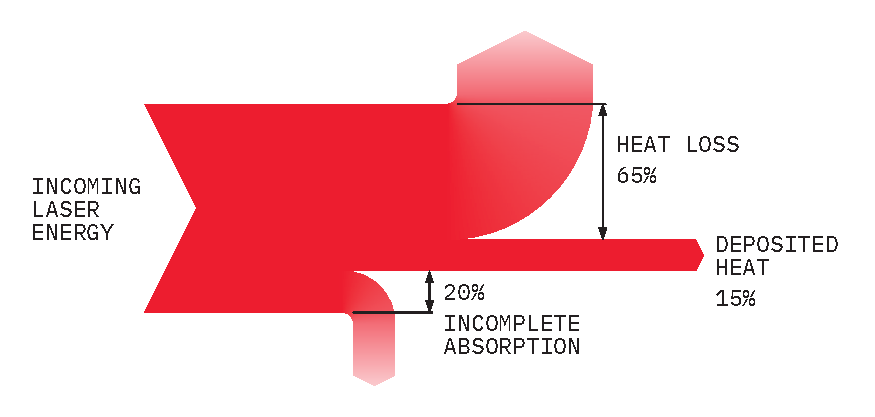
\includegraphics[]{assets/5 results/heatdep_contribs.pdf}
                \caption{Major losses in the overall heat deposition. Diagram to scale.}
                \label{fig:heatdep_sankey}
            \end{figure}

            Although useful to estimate heat deposition, the assumption of uniform distribution of heat in the test section does not accurately reflect the actual processes taking place during LSP growth and shortly afterward. This simplifying assumption does not explain the intermediate rise in pressure followed by a short drop immediately after the end of the laser pulse.

            This simple method of determining heat deposition and its efficiency could also be improved on in a few ways. First, replicating these experiments using (a more reliable) spark-ignition system would likely mitigate any heat transfer (although already estimated to be small) occurring via the ignition system. This would also allow the LSP to extend downstream past the ignition point, which may have implications on both laser absorption and overall heat deposition. Second, heat transfer to the walls should be quantified to determine whether this would explain the observed pressure drop after the (global) maximum, and to correct, if deemed necessary, for heat transfer to the walls as the gas is heating up. These changes would likely improve the calculated heat-deposition efficiency.
    \newpage
    \section{Spectroscopic temperature measurement} \label{sec:results_spectroscopy}
        Spectral data was acquired for several LSP tests, at \qty{20}{bar} and \qty{10}{bar} and varying laser power settings. Only one spectral measurement was performed during a test. No collimator was mounted to the fiber termination, allowing the spectrometer to sample a relatively large field of view of the experiment, rather than a single point on the plasma. The sampling area was determined to be approximately \qty{4}{cm} in diameter at the location of the LSP. This simplified alignment procedures as some part of the LSP's emission was practically guaranteed to be captured by the fiber, and it was assumed that the emitted radiation from the hottest part of the plasma would dominate over that of cooler regions.

        \autoref{fig:spectrum_lines} shows the captured spectral data from an LSP at \qty{20}{bar} and \qty{3}{kW} of laser power. Ar~I emission lines are clearly visible and closely match the lines tabulated by NIST~\cite{kramidaNISTAtomicSpectra2022}. Continuum radiation and Ar~II emission lines are also seen in the 400--600-nm region, exhibiting the same features seen in spectra captured by \textcite{luCharacteristicDiagnosticsLaserStabilized2022}. However, unlike \citeauthor{luCharacteristicDiagnosticsLaserStabilized2022}'s data, the captured spectrum shows a drastic difference between the intensity of continuum radiation compared to the Ar~I line emissions, almost by an order of magnitude. \added{For instance, the magnitude of the 811-nm line relative to the peak of the continuum radiation ($\sim$500~nm) in \citeauthor{luCharacteristicDiagnosticsLaserStabilized2022}'s data is around 5. As seen in \autoref{fig:spectrum_lines}, that ratio is closer to 20 for this project's data. Considering their plasmas were sustained with a 200~W laser, a possible explanation could lie in the difference in laser power magnitude. Not enough spectral data was acquired at comparable power levels to confirm this, however.}

        \begin{figure}[h]
            \centering
            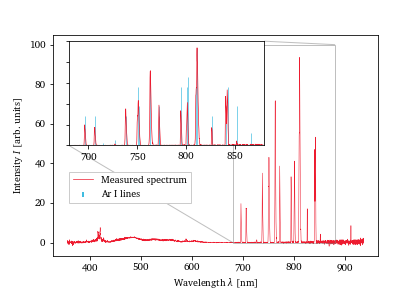
\includegraphics[]{assets/5 results/spectrum_LSP50_X7_lines}
            \caption{Detection of Ar I emission lines in \texttt{LSP50\_X7} in static argon}
            \label{fig:spectrum_lines}
        \end{figure}
        \newpage
        \subsection{Boltzmann plot method}
            Temperature calculation can be performed from spectral data using the Boltzmann plot method, summarized by \textcite{ohnoValidityElectronTemperature2006} and discussed in further detail by \textcite{griemSpectroscopicTemperatureMeasurements1997}. The transition of an electron from an upper atomic energy level $k$ to a lower level $i$  generates an emission line at wavelength $\lambda_{ki}$ with transition probability $A_{ki}$ and degeneracy for level $k$ of $g_k$. The following equation can be derived to relate these parameters to plasma temperature $T$:
            \begin{equation} \label{eq:transition_energy}
                \frac{\epsilon_{ki}\lambda_{ki}}{A_{ki}g_k} = \frac{\hbar cn}{2 \mathcal{Z}(T)}\exp{\left(-\frac{E_k}{k_\mathrm{B}T}\right)}
            \end{equation}
            Where $c$ is the speed of light, $n$ is the atomic number density, $\mathcal{Z}(T)$ is the partition function, and $\epsilon_{ki}$ is the spectrally integrated emission line intensity. This equation can be linearized with respect to $E_k$ by taking the natural log of both sides:
            \begin{equation} \label{eq:boltzmannplot}
                \ln{\frac{\epsilon_{ki}\lambda_{ki}}{A_{ki}g_k}} = -\frac{E_k}{k_\mathrm{B}T} + \ln{\frac{\hbar cn}{2 \mathcal{Z}(T)}}
            \end{equation}
            The second term is a constant for a given temperature, so $E_k$ can be plotted against the left-hand side of \autoref{eq:boltzmannplot}, resulting (in theory) in a straight line with gradient $-1/k_\mathrm{B}T$. This can then be used to evaluate $T$. However, as noted by \textcite{volkerImportancePhysicalUnits2022}, $\epsilon_{ki}\lambda_{ki}/A_{ki}g_k$ is not dimensionless, and a measure of absolute emission intensity can only be done with appropriate spectrometer calibration, which was not done in this study. There are several methods to resolve these issues, including one that can be used with the relative spectrometry data of this project. This ratio can be normalized by using a reference transition, denoted with the subscript $r$\added{. The reference transition functions as a datum and can be arbitrarily selected from the transitions observed in the spectrum, as long as it is consistently used for each data point.}
            \begin{equation} \label{eq:reference_transition}
                \left[\frac{\epsilon_{ki}\lambda_{ki}}{A_{ki}g_k}\right]_\mathrm{r} = \frac{\hbar cn_\mathrm{r}}{2 \mathcal{Z}_\mathrm{r}(T)}\exp{\left(-\frac{E_k}{k_\mathrm{B}T}\right)_\mathrm{r}}
            \end{equation}
            Multiplying either side of the original equation by the reciprocal of the above, then linearizing, yields the following, with the constant term bundled as $C$:
            \begin{equation}
                \ln{\left(\frac{\epsilon_{ki}\lambda_{ki}}{A_{ki}g_k}\left[\frac{A_{ki}g_k}{\epsilon_{ki}\lambda_{ki}}\right]_\mathrm{r}\right)} = \frac{-E_k+[E_k]_\mathrm{r}}{k_\mathrm{B}T} + C
            \end{equation}
            This normalization enables a temperature to be determined using relative spectral data, as they are all compared to the same reference line in the spectrum. This manipulation has no effect on the gradient of the plot.

        \subsection{Temperature calculation}
            The acquired spectral data for LSP was processed to extract temperature data using the Boltzmann plot method discussed in the previous section. A subset of emission lines strong enough to be consistently observed for all tests, and well separated from other lines to facilitate identification and spectral integration were selected for this analysis. Relevant properties for these transitions were acquired from the NIST Atomic Spectra Database~\cite{kramidaNISTAtomicSpectra2022} and are tabulated for the selected lines in \autoref{tab:ArI_transitions}. The emission coefficients $\epsilon_{ki}$ were computed by fitting a Voigt line profile to the measured spectral lines, and integration was performed on the fitted curve. The \num{763.51}-\unit{nm} transition was used as the reference line.

            \begin{table}[h]
                \centering
                \caption[Ar I transitions used to generate Boltzmann plot]{Ar I transitions used to generate Boltzmann plot. The transition wavelength is $\lambda_{ki}$, $g_k$ is the degeneracy of the energy level $k$, $A_{ki}$ the transition probability from level $k$ to $i$, $\Delta A_{ki}/A_{ki}$ is the relative uncertainty of $A_{ki}$, and $E_k$ is the energy of level $k$. Taken from \textcite{kramidaNISTAtomicSpectra2022}.}
                \label{tab:ArI_transitions}
                \begin{tabular}{@{}Srrr@{}}
                    \toprule
                    $\lambda_{ki}$ [nm] & $g_kA_{ki}$ [\unit{s^{-1}}] & $\Delta A_{ki}/A_{ki}$ [-] & $E_k$ [eV]  \\ \midrule
                    696.54         & \num{1.90E+07}                    & 0.07                       & 13.328 \\
                    706.72         & \num{1.90E+07}                    & 0.10                       & 13.302 \\
                    738.40         & \num{4.20E+07}                    & 0.10                       & 13.302 \\
                    763.51         & \num{1.22E+08}                    & 0.10                       & 13.172 \\
                    794.82         & \num{5.58E+07}                    & 0.10                       & 13.283 \\
                    826.45         & \num{4.59E+07}                    & 0.07                       & 13.328 \\ \bottomrule
                \end{tabular}
            \end{table}

            \highlight[id=BZ, comment=What is the temperature calculated per point (...)?]{Sample Boltzmann plots}\comment[id=ED]{Calculating this requires knowledge of $n$ which also depends on $T$} generated from LSP with \num{20.14}-\unit{bar} argon at \qty{3.08}{kW} are shown in \autoref{fig:boltzmannplot}. It is immediately apparent that the data points are very loosely correlated, providing low confidence in the resulting temperature, which was calculated to be \qty{8000}{K}\added{ and \qty{5000}{K}}. This does not appear possible, as ionization calculations such as the ones done in \autoref{sec:models_absorption} suggest argon is not in a plasma state at these temperatures, and that little to no free electrons are available to absorb radiation via inverse bremsstrahlung. \added{Although other absorption mechanisms exist, none appear likely to absorb 1070-nm laser radiation. Bound-bound electronic energy transitions in Ar~I do not feature a 1070-nm band. Absorption lines exist at \qty{1068.3}{nm} and \qty{1073.4}{nm}, but they are faint ($g_kA_{ki}\sim$ 10$^5$~\unit{s^{-1}})~\cite{kramidaNISTAtomicSpectra2022}. Bound-free transitions (photoionization) would require photons with enough energy to ionize argon. The energy $E$ of a photon can be calculated by \autoref{eq:planck-einstein}, the Planck--Einstein relation:}
            \begin{equation} \label{eq:planck-einstein}
                E = \frac{2\pi \hbar c}{\lambda}
            \end{equation}
            \added{Evaluating \autoref{eq:planck-einstein} for 1070-nm radiation yields \qty{1.16}{eV}, less than the 15.76-eV ionization energy of Ar~I. Only UV and shorter-wavelength radiation carry sufficient energy. }\replaced{Another factor undermining the confidence in these temperature values is their sensitivity to the subset of data used in the calculation:}{Furthermore,} the selection of a different set of transition lines results in major variations in the computed temperature, sometimes suggesting negative absolute temperatures (characterized by a positive slope on the plot). \added{Given these inconsistencies, few conclusive observations can be made from this spectroscopic analysis.}\comment[id=BZ]{Can you explain why temperature is higher at high pressure?}\comment[id=ED]{I have very little trust in these temperature measurements so I cannot say}
            
            \begin{figure}[h]
                \centering
                \begin{subfigure}[t]{0.47\textwidth}
                    \centering
                    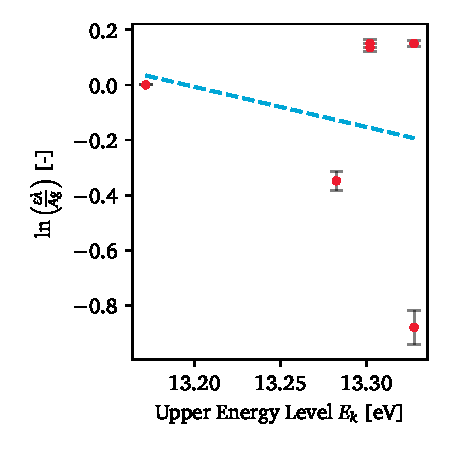
\includegraphics[width=\textwidth]{assets/5 results/spectrum_LSP50_X7_boltzmann}
                    \caption{\qty{20}{bar}, \texttt{LSP50\_X7}: $T \approx$ \qty{8000}{K}}
                    \label{fig:boltzmann_LSP50_X7}
                \end{subfigure}
                \hfill
                \begin{subfigure}[t]{0.47\textwidth}
                    \centering
                    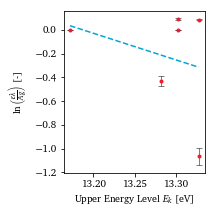
\includegraphics[width=\textwidth]{assets/5 results/spectrum_LSP60_S9_boltzmann}
                    \caption{\qty{10}{bar}, \texttt{LSP60\_S9}: $T \approx$ \qty{5000}{K}}
                    \label{fig:boltzmann_LSP60_S9}
                \end{subfigure}
                \caption{Boltzmann plots of selected LSP sustained at \qty{3}{kW}}
                \label{fig:boltzmannplot}
            \end{figure}

            There may be several reasons for this poor accuracy. The first is that the upper energy levels $E_k$ of most Ar I emission lines are clustered near \qty{13.25}{eV}, providing a poor sampling range for a linear regression. This is often the case when considering the relative line intensities only for a given atom or ion, as pointed out by \textcite{griemSpectroscopicTemperatureMeasurements1997}: excitation energies are often clustered together. This could be improved 
            % in two ways: the \num{750.39}-\unit{nm} transition of Ar I has an excitation energy of \qty{14.95}{eV}, significantly greater than the other transitions. However, its closeness to the \num{751.47}-\unit{nm} transition requires more sophisticated processing to discriminate its emission contribution from that of its neighboring line. Alternatively, a line emission of Ar I could be compared 
            by comparing an Ar I line to an Ar II line. This however requires knowledge of electron density, and a measure of Ar II emission lines. These lines are present in the experimental data, in the range of \qtyrange{400}{500}{nm}, but are much fainter than the Ar I lines, far more clustered together, and blended into the continuum radiation of the plasma, making detection and integration difficult.

            Another possible factor for poor temperature results is that the spectrometer fiber sampled a relatively large area in the test section, and that contrary to the assumption made before this experiment, the emitted radiation of the hottest parts of the LSP do not dominate over colder areas, at least not for the emission lines.  \textcite{nassarInvestigationLasersustainedPlasma2012} used a collimator to sample the spectrum from specific points in the plasma and had better success in determining temperature. 
    
    \section{Flowing experiments} \label{sec:exp_flowing}
        To inform the design and test of dedicated thruster prototypes, the test section of this study was also designed such that it could be configured for flowing/thruster operation, by replacing the downstream end of the system with a backplate featuring an NPT-threaded port onto which various small nozzles could be inserted. Both the effects of forced flow on LSP properties, and the resulting thrust were of interest. Unlike some of the experiments discussed in \autoref{sec:background_exp}, it should be noted no attempt was made at straightening the flow or quantifying its uniformity, as the test section did not provide an easy way to do this. This configuration is illustrated in \autoref{fig:finalsetup_flowing}. Due to the use of an opaque nozzle module, the power meter could no longer be used for absorption measurements. The facility was fitted on a thrust stand to attempt to measure any changes in the thrust of the apparatus due to the LSP.

        \begin{figure}[h]
            \centering
            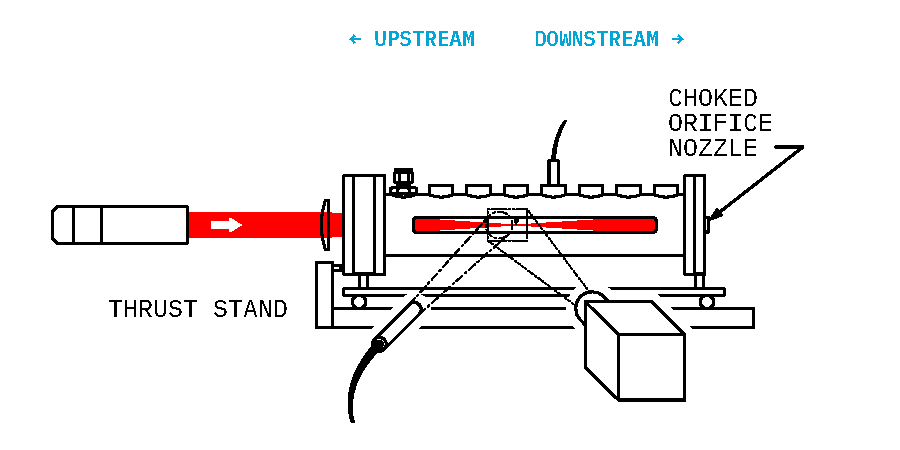
\includegraphics[width=0.85\textwidth]{assets/5 results/finalsetup_flowing}
            \caption{Flowing configuration of the test section}
            \label{fig:finalsetup_flowing}
        \end{figure}

        Flow rate was controlled by a delivery pressure set by a regulator and choked orifice nozzles of varying diameter, made by drilling out blank NPT plugs. The test section static pressure was set such that choking conditions could be guaranteed, i.e., the ambient pressure was lower than the sonic pressure. This allows the calculation of the mass flow rate using \autoref{eq:massflow}.
        % \footnote{Equivalent to Equation 6-6 in \citeauthor{zandbergenAE4S01ThermalRocket2020}'s \citetitle*{zandbergenAE4S01ThermalRocket2020} course notes~\cite{zandbergenAE4S01ThermalRocket2020}},\added{ derived from the choked (critical) mass flow rate equation assuming a circular orifice,} with the orifice nozzle throat area $D_\mathrm{t}$, stagnation pressure $p_0$, and stagnation temperature $T_0$.
        % \begin{equation}
        %     \dot{m} = \sqrt{\frac{\gamma}{R_\mathrm{g}}\left(\frac{2}{\gamma+1}\right)^\frac{\gamma+1}{\gamma-1}}\frac{A_\mathrm{t}p_0}{\sqrt{T_0}} = K_{\dot{m}}\frac{A_\mathrm{t}^2p_0}{\sqrt{T_0}} \tag{\ref{eq:massflow} revisited}
        % \end{equation}
        % For the temperatures of interest in the overall flow (excluding the LSP), $K_{\dot{m}}$ for argon is \qty{0.0504}{s.K^{1/2}.m^{-1}}. \added{For those familiar with the Vandenkerckhove function $\Gamma$, the mass flow parameter $K_{\dot{m}}$ is equivalent to $\Gamma/R_\mathrm{g}^{1/2}$.} 
        Assuming incompressible conditions in the test section, the bulk fluid velocity $v_\mathrm{c}$ can be determined from \autoref{eq:massflow} and conservation of mass, resulting in \autoref{eq:bulk_fluid_vel}, where $D_\mathrm{c}$ is the test section internal diameter (\qty{1.5}{in}).
        \begin{equation} \label{eq:bulk_fluid_vel}
            v_\mathrm{c} = K_{\dot{m}}\frac{D_\mathrm{t}^2}{D_\mathrm{c}^2}R_\mathrm{g}\sqrt{T_0}
        \end{equation}
        Relatively large nozzle sizes were used to force flow in the test sections at speeds on the same order as the LSP growth speed ($\sim$~\qty{10}{m.s^{-1}}), to determine the LSP could be modified or blown out by fast enough flows. This is relevant for the thrust chamber design of an LTP thruster, as this could place constraints on the chamber dimensions. Unfortunately, the maximum nozzle diameter was limited to about \qty{4}{mm}, as this was the feed system's internal diameter. Using larger nozzles would have resulted in choking at the inlet, capping the mass flow rate (and test section flow velocity). The available nozzles under this diameter \added{theoretically} provided \deleted{a} bulk flow velocit\added{ies and mass flow rates tabulated in \autoref{tab:nozzlespec}. The resulting flow speeds in the test section are relatively low and may not reflect those of a dedicated thruster prototype}.

        \begin{table}[h]
            \centering
            \caption[Specifications for choked orifice nozzles used for flowing tests]{Specifications for choked orifice nozzles used for flowing tests, for \qty{10}{bar} of test section pressure. The nozzle diameter $D$, test-section bulk flow velocity $v_\mathrm{c}$, and mass flow rate $\dot{m}$ are given.}
            \label{tab:nozzlespec}
            \begin{tabular}{SSS}
                \toprule
                {$D$ [mm]} & {$v_\mathrm{c}$ [\unit{m.s^{-1}}]} & {$\dot{m}$ [\unit{g.s^{-1}}]} \\
                \midrule
                2.67	& 0.88	& 16.5  \\
                3.05	& 1.15	& 21.5  \\
                3.81	& 1.80	& 33.6  \\
                \bottomrule
            \end{tabular}
        \end{table}

        \autoref{fig:flow_v_static} compares the LSP size between the static and flowing case. What is apparent is a noticeably slower growth of the LSP in the upstream direction, suggesting that the forced flow does affect LSP dynamics. The upstream tip of the flowing LSP settles closer to the ignition point than for the static LSP. Forced flow also appears to help the LSP sever the ignition wire, allowing it to extend further past the ignition point, which was not always the case in static conditions. While the overall length of the flowing LSP is longer, it may not be appropriate to compare it to the static case as the wire prevents downstream growth.

        \begin{figure}[h]
            \centering
            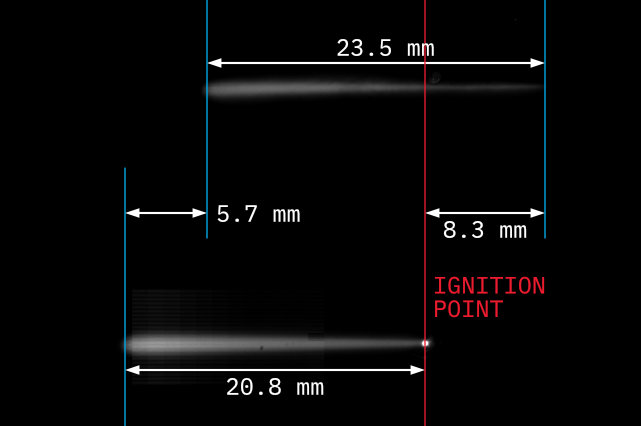
\includegraphics[]{assets/5 results/flow_static_lsp.jpg}
            \caption[Comparison of LSP under forced flow (top) and static LSP (bottom)]{Comparison of LSP under forced flow (top) and static LSP (bottom). \qty{10}{bar}, \qty{3080}{W}, the bulk flow velocity was \qty{1.8}{m.s^{-1}}}
            \label{fig:flow_v_static}
        \end{figure}

        Although bulk flow velocities capable of blowing out the LSP were not attained, LSP stability was observed to be susceptible to flow conditions. As seen in \autoref{sec:background_exp}, past LTP facilities such as those of \textcite{toyodaThrustPerformanceCW2002} had features to distribute flow evenly in the test section with little turbulence. This was not the case in this project, as the gas was injected from a single orifice a few inches upstream of the LSP, through the side of the test section rather than co-axially. This likely results in flow with significant, unsteady, rotational and/or radial velocity components by the time it reaches the LSP. Disturbances to the LSP were observed, such as dissipation before the end of the laser pulse, separation of one LSP into two cores, which could sometimes reconnect, and localized variations in plasma brightness during a laser pulse.

        \autoref{fig:flow_pressure} presents the acquired pressure data for some flowing tests, including heat-deposition efficiency calculations. The pressure profile matches the same pattern observed in static conditions. Although the data suggests a slightly lower heat deposition compared to the static case, the sample size is small, and the flow velocities remain low, almost comparable to static conditions. Definite conclusions based on this limited data may thus be premature. \added{Furthermore, as stated earlier, experiments by \textcite{mazumderSpectroscopicStudiesPlasma1987} suggest that increased flow rates result in improved heat deposition efficiencies. As their results were obtained at flow rates of 2--10~\unit{m.s^{-1}}, it may be that greater flow rates are necessary to observe a significant and consistent change in heat deposition efficiency.} Nevertheless, one noticeable and consistent difference between the static and flowing cases is the intermediate pressure maximum---it appears to be 40\% greater than in the static case. 

        Spectral data was acquired for flowing tests, but exhibited little difference compared to spectra acquired at comparable pressures under static conditions.

        \begin{figure}[h]
            \centering
            \begin{subfigure}[t]{0.47\textwidth}
                \centering
                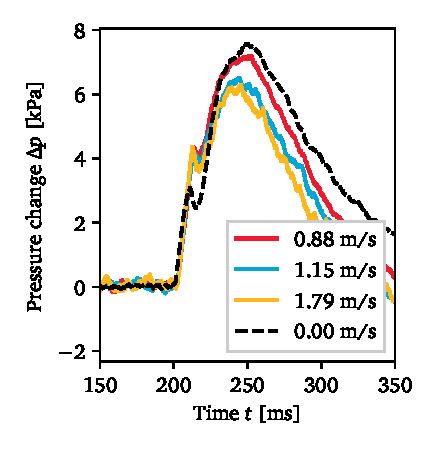
\includegraphics[width=\textwidth]{assets/5 results/flow_deltap}
                \caption{Pressure rise}
                \label{fig:flow_pressure_rise}
            \end{subfigure}
            \hfill
            \begin{subfigure}[t]{0.47\textwidth}
                \centering
                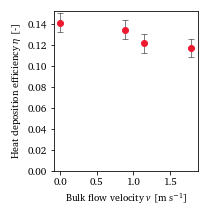
\includegraphics[width=\textwidth]{assets/5 results/flow_eta}
                \caption{Calculated heat-deposition efficiency}
                \label{fig:flow_pressure_efficiency}
            \end{subfigure}
            \caption[Pressure change and heat-deposition efficiency in flowing LSP]{Pressure change and heat-deposition efficiency in flowing LSP. \qty{10}{bar}, \qty{30.6}{J} input energy.}
            \label{fig:flow_pressure}
        \end{figure}